\chapter{Hybrid Task Manager for Interactive Workloads}
\label{chapter: hipster}

%Previous chapter

\looseness -1 \lettrine{I}{n} the previous chapters, we introduced a framework to
estimate performance and power consumption of batch workloads using a statistical
modelling technique. By contrast, this chapter focuses on an application-level scheduling
approach for latency-critical and batch workloads, by taking advantage of processor
capabilities (like OS-level DVFS)~\citep{WonyoungKim2008SystemRegulators,
Godycki2014EnablingNetworks, Putnam2014AServices, Lo2014DynamicChips} to improve energy
efficiency or resource utilisation.  Collocating latency-critical with batch workloads is
interesting because the former is striving to deliver a service within a certain
quantum~\citep{Barroso2013TheEdition}, whereas the latter is aimed at maximising
performance.

%Importance of EF, and new computing

%\looseness -1 Maintaining energy efficiency in large scale data centres is, in fact, one
%of the most important problem of this decade and modern systems have been exploring
%alternative heterogeneous processors~\citep{Halpern2016MobileSatisfaction,
%Wong2012KnightShift:Heterogeneity, Chitlur2012QuickIA:Prototypes,
%Guevara2013NavigatingMechanisms, Mars2011HeterogeneityOpportunity,
%Cong2012Energy-efficientArchitectures, DBLP:journals/ppl/VillebonnetCLPS15} and DVFS to
%trade-off performance and power.

%Need for QoS metric 

\looseness -1 Many important cloud workload are latency-critical, and require strict levels of QoS to
meet SLA requirements~\citep{Lo2015Heracles, Kasture2015Rubik, Lo2014TowardsWorkloads}.
For instance, a web-request must complete within a certain time frame otherwise users are
likely to leave.  Recent study has shown that marginal delays in QoS (of hundreds of
milliseconds) can impact revenue massively~\citep{Eric2009TheSearch}. In particular it is
important to meet QoS tail latency, such as \ninefive or \ninenine percentile of request
latency distribution~\citep{Dean2013TheScale}.

%Traditional schedulers are not suitable.

\looseness -1 Recent works~\citep{Petrucci2015Octopus-Man:Computers, Lo2015Heracles, Kasture2015Rubik,
Delimitrou2013Paragon:Datacenters, Vamanan2015TimeTrader:Search, Zhu2016Dirigent} have shown that
traditional power management practices and CPU utilisation measures are unsuitable to
drive task management for data centre workloads.  This is because prior schemes (like
OS-level DVFS) work well to deliver long-term performance for batch workloads, but they
can severely hurt the QoS of latency-critical data centre workloads. 

%Need for corunning

\looseness -1 As noticed in prior work~\citep{Petrucci2015Octopus-Man:Computers, Lo2015Heracles,
Kasture2015Rubik, Delimitrou2013Paragon:Datacenters, Vamanan2015TimeTrader:Search,
Zhu2016Dirigent}, workload management can be very challenging in heterogeneous server
systems because an application can experience different behaviour in QoS and resource
efficiency depending on specific resource allocation decisions. This requires careful
resource characterisation of the running workloads to optimise resource usage. In many
data centres, there also is a wish to run both latency-critical and batch workloads.
Running both latency-critical and batch workloads, in this way, increases cluster
utilisation during periods of low demand, reducing operational cost and total energy
consumption.

\looseness -1 Precisely, we introduce \textbf{Hipster}, a scheme that manages
heterogeneous \muc allocation and DVFS settings for latency-critical workloads given QoS
constraints, while minimising system power consumption. In addition, Hipster allows
collocation of latency-critical and batch workloads in shared data centres to maximise the
data centre utilisation. In such scenarios, the resources allocated to latency-critical
workloads are just enough to meet the QoS target, and the remaining resources are
allocated to throttle the batch workloads.

The major contributions of this chapter are: 

\looseness -1 {\small\circled{1}} We present \textbf{Hipster}, a hybrid management
solution combining  heuristic techniques and reinforcement learning to make
resource-efficient allocation decisions, specifically deciding the best mapping of
latency-critical and batch workloads on heterogeneous cores (big and small) and their DVFS
setting (Section~\ref{sec: methodology-hipster}).

\looseness -1 {\small\circled{2}} Hipster is presented in two variants: \textbf{HipsterIn} and
\textbf{HipsterCo}. HipsterIn (for interactive workloads) is targeted towards allocating
resources to latency-critical workloads so that the system power consumption is minimised,
whereas HipsterCo (for collocated workloads)  enables running both latency-critical and
batch workloads for improved server utilisation. Both variants ensure that QoS for
latency-critical workloads is met.  

{\small\circled{3}} We carried out real measurement experiments on a 64-bit big-LITTLE
(ARM Juno R1) platform along with back-end services such as Web-Search and Memcached. The
request generator for each of the back-end services follows a diurnal load pattern typical
of production data centres (Section~\ref{sec: architecture}).  


{\small\circled{4}} We evaluate Hipster against the only other heterogeneous
platform-aware state-of-the-art scheme~\citep{Petrucci2015Octopus-Man:Computers} that
dynamically allocates heterogeneous cores to latency-critical workloads. Our results show
that HipsterIn outperforms prior work, in energy consumption reduction by 13\%, while
achieving up to 99\% QoS guarantees for the latency-critical workloads. In addition, our
results for HipsterCo show that it improves performance by $2.3\times$ compared to a
static/conservative policy running batch workloads, while meeting QoS targets for
latency-critical workloads (Section~\ref{sec: evaluation-hipster}).

{\small\circled{5}} We evaluate the ability of our scheme to adapt dynamically to changes
in application at runtime. Our results show that HipsterIn can adapt to changes in
application, while achieving up to 98\% QoS guarantees for the latency-critical workloads.
Finally, we present the source code written in Python for Hipster that can be used to
deploy different cloud workloads such as Web-Search and Memcached. 



\iffalse

\looseness -1 We begin this chapter by motivating the need for a new scheduler
(Section~\ref{sec:Motivation}) by identifying the flaws in the existing state-of-the-art.
Next, we present \textbf{Hipster} (), which is a hybrid management solution combining
heuristic techniques and reinforcement learning (RL) to make resource-efficient allocation
decisions, specifically deciding the best mapping of latency-critical and batch workloads
on heterogeneous cores (big and small) and their DVFS setting. Hipster is presented in two
variants: \textbf{HipsterIn} and \textbf{HipsterCo}. 

\looseness -1 Thereafter, we describe HipsterIn (for interactive workloads) is targeted towards
allocating resources to latency-critical workloads so that the system power consumption in
minimised.  Followed by HipsterCo (for collocated workloads)  which enables running both
latency-critical and batch workloads for improved server utilisation. Both variants ensure
that QoS for latency-critical workloads is met. 

\looseness -1 The results for Hipster were carried real measurement experiments using a 64-bit
big.LITTLE (ARM Juno R1) platform along with back-end services such as Web-Search and
Memcached. The request generator for each of the back-end services follows a diurnal load
pattern typical of production data centres. The description of the ARM processor is given
in .

\looseness -1 Next, we evaluate  Hipster against the only other \het platform-aware
state-of-the-art scheme~\citep{Petrucci2015Octopus-Man:Computers} that dynamically
allocates \het cores to latency-critical workloads, and show that our scheduling algorithm
out-performs the state-of-the-art scheme.

\looseness -1 Finally, we evaluate the ability of our scheme to adapt dynamically to changes in
application at runtime. Our results show that HipsterIn can adapt to changes in
application, while achieving up to 98\% QoS guarantees for the latency-critical workloads.
Finally, we present the source code written in Python for Hipster that can be used to
deploy different cloud workloads such as Web-Search and Memcached.  

\fi

\nomenclature[z-RL]{$RL$}{Reinforcement learning}


\section{Motivation}
\label{sec:Motivation}

Typical web applications experience large variations in user traffic over
time.\footnote{Roy \etal~\citep{Roy:2015:ISN:2785956.2787472} and Bronson
\etal~\citep{180185} show network bytes over the course of the day for a web-server and
memcached~\citep{Nishtala2013ScalingFacebook} at Facebook.}
Figure~\ref{fig:websearchmotivation}, for example, shows how the number of queries per second during a web search, 
a typical load at Google data centre, varies between about
\SI{5}{\percent} and \SI{80}{\percent} of maximum capacity~\citep{Hoelzle2009TheMachinesb,
Meisner2011PowerServices,Lo2014TowardsWorkloads}.  Similarly, Facebook consistently sees
diurnal load variations between \SI{10}{\percent} and \SI{95}{\percent} of maximum
capacity, across multiple server clusters~\citep{Bilgir_exploringthe,
Atikoglu2012WorkloadStore}.

\begin{figure}[ht]
	\centering
    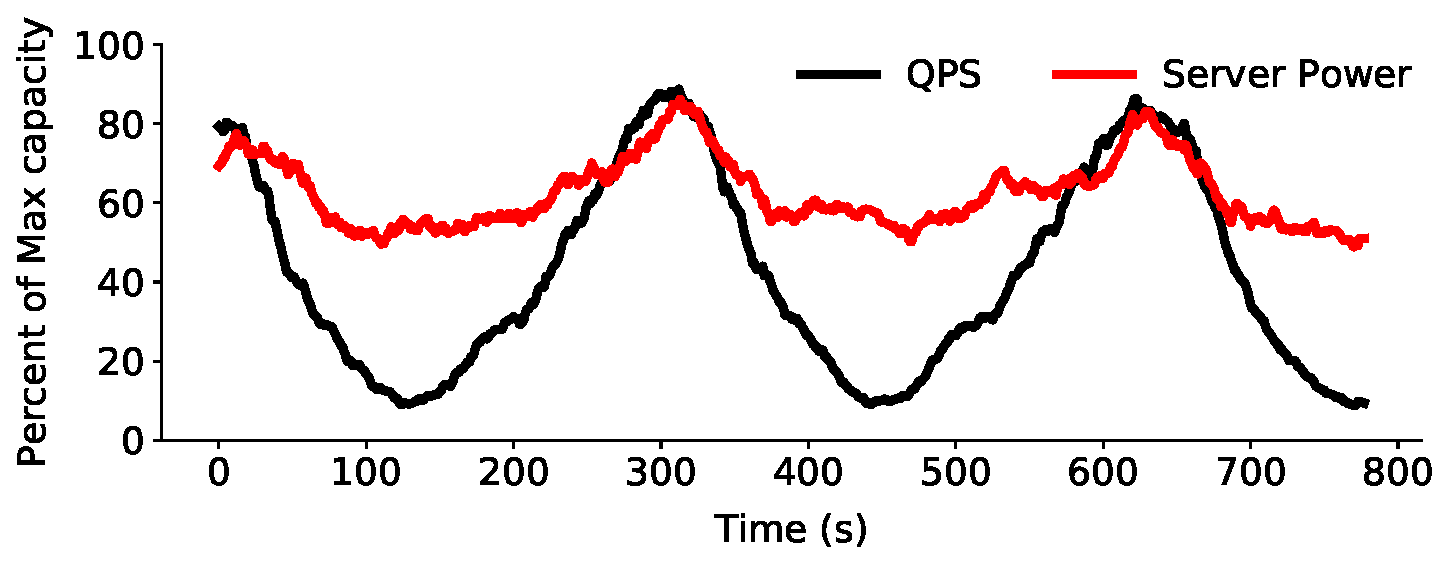
\includegraphics[width=\textwidth]{Chapter4/Figs/google_trace.eps}
    \caption[Power drawn for a diurnal load]{\captitle{Power drawn for a diurnal load~\citep{Meisner2011PowerServices,Lo2014TowardsWorkloads,Hoelzle2009TheMachinesb}.} The power consumption is measured for Web-Search running on two big cores of the ARM Juno R1 (64-bit big.LITTLE) platform.}
	\label{fig:websearchmotivation}
\end{figure}


The periods of low server utilisation provide opportunity to reduce data centre energy
consumption~\citep{Petrucci2015Octopus-Man:Computers, Lo2015Heracles,
Delimitrou2013Paragon:Datacenters, Delimitrou:2013:QSH:2542150.2556583}. As seen in
Figure~\ref{fig:websearchmotivation}, although load drops dramatically, power consumption
is always at \SI{60}{\percent} or above.  For this reason, both academia and industry are
working towards better energy proportionality; i.e. that the system's power consumption is
proportional to utilisation.

There are also opportunities to improve energy efficiency using heterogeneous servers
combined with DVFS. Heterogeneous servers can minimise power consumption at low load by
deploying small cores, and can provide maximum performance using big cores to meet the QoS
target for latency-critical workloads~\citep{Petrucci2015Octopus-Man:Computers,
JanapaReddi2010WebCores, Chitlur2012QuickIA:Prototypes}.

\paragraph{Mixing different core types with DVFS.} Figure~\ref{fig:octomancomp} shows the
energy efficiency in RPS/Watt and QPS/Watt when using a state-of-the-art baseline
policy~\citep{Petrucci2015Octopus-Man:Computers}.\footnote{Recall, RPS refers to requests
per second and QPS refers queries per second (see section~\ref{sec: perfmon thesis})} We
explore a heterogeneous architecture mixing different core types and DVFS (HetCMP) 

\begin{figure}[htbp]
\begin{subfigure}{\textwidth}
  \centering
  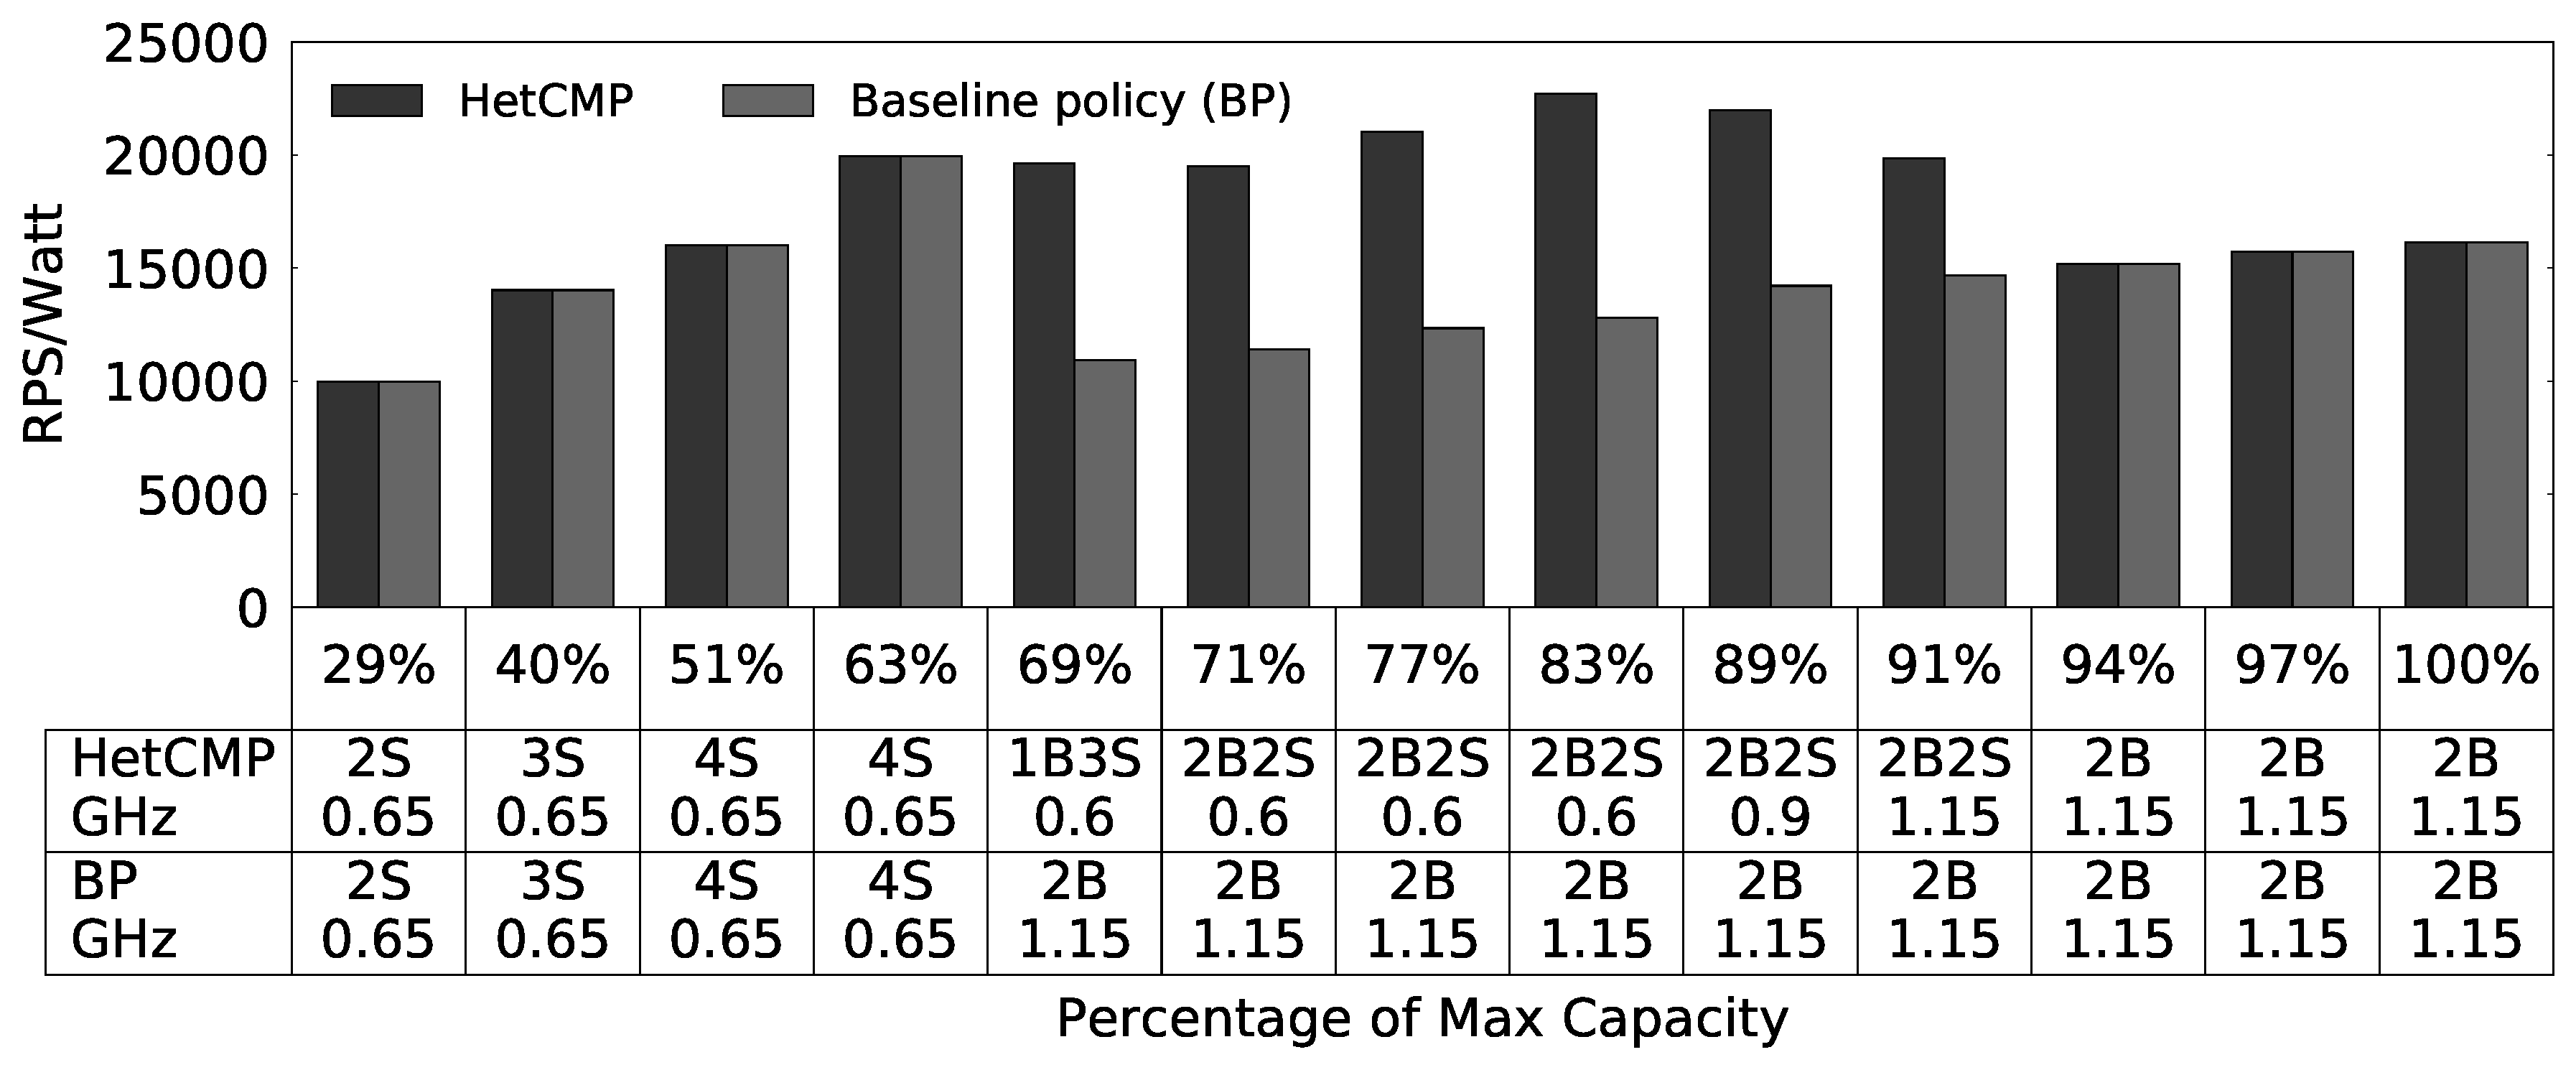
\includegraphics[width=0.9\linewidth]{Chapter4/Figs/rps-watt-memcached.eps}
  \caption{Memcached}
  \label{fig: improvements}
\end{subfigure}
%\hspace{-2.8em}
\begin{subfigure}{\textwidth}\ContinuedFloat
  \centering
  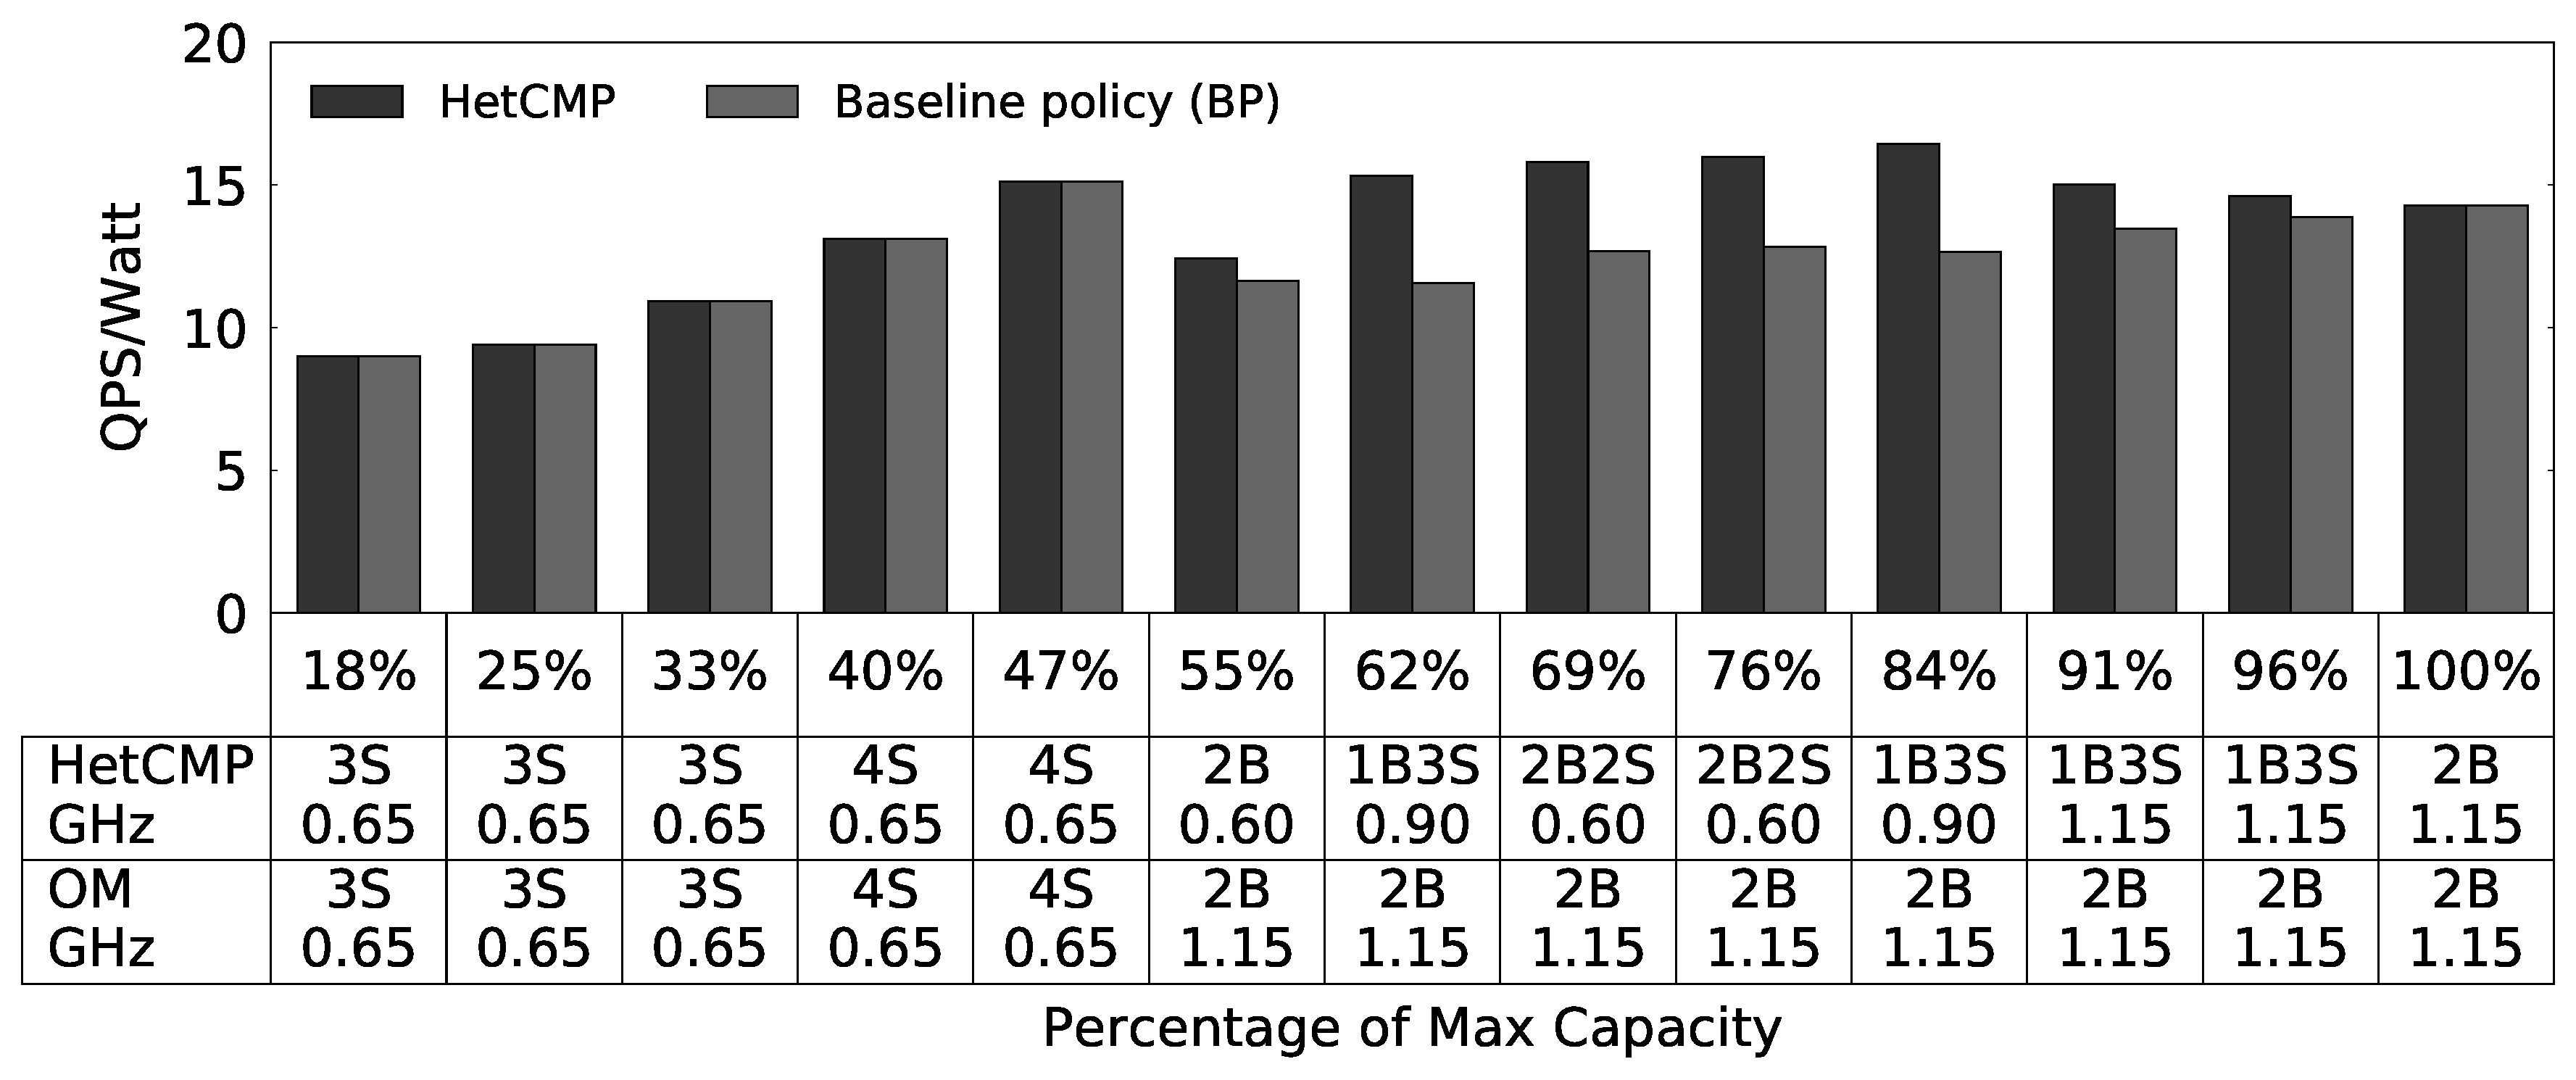
\includegraphics[width=0.9\linewidth]{Chapter4/Figs/rps-watt-websearch-new.eps}
  \caption{Web-Search}
  \label{fig: improvements-websearch}
\end{subfigure}
\begin{subfigure}{\textwidth}\ContinuedFloat
  \centering
  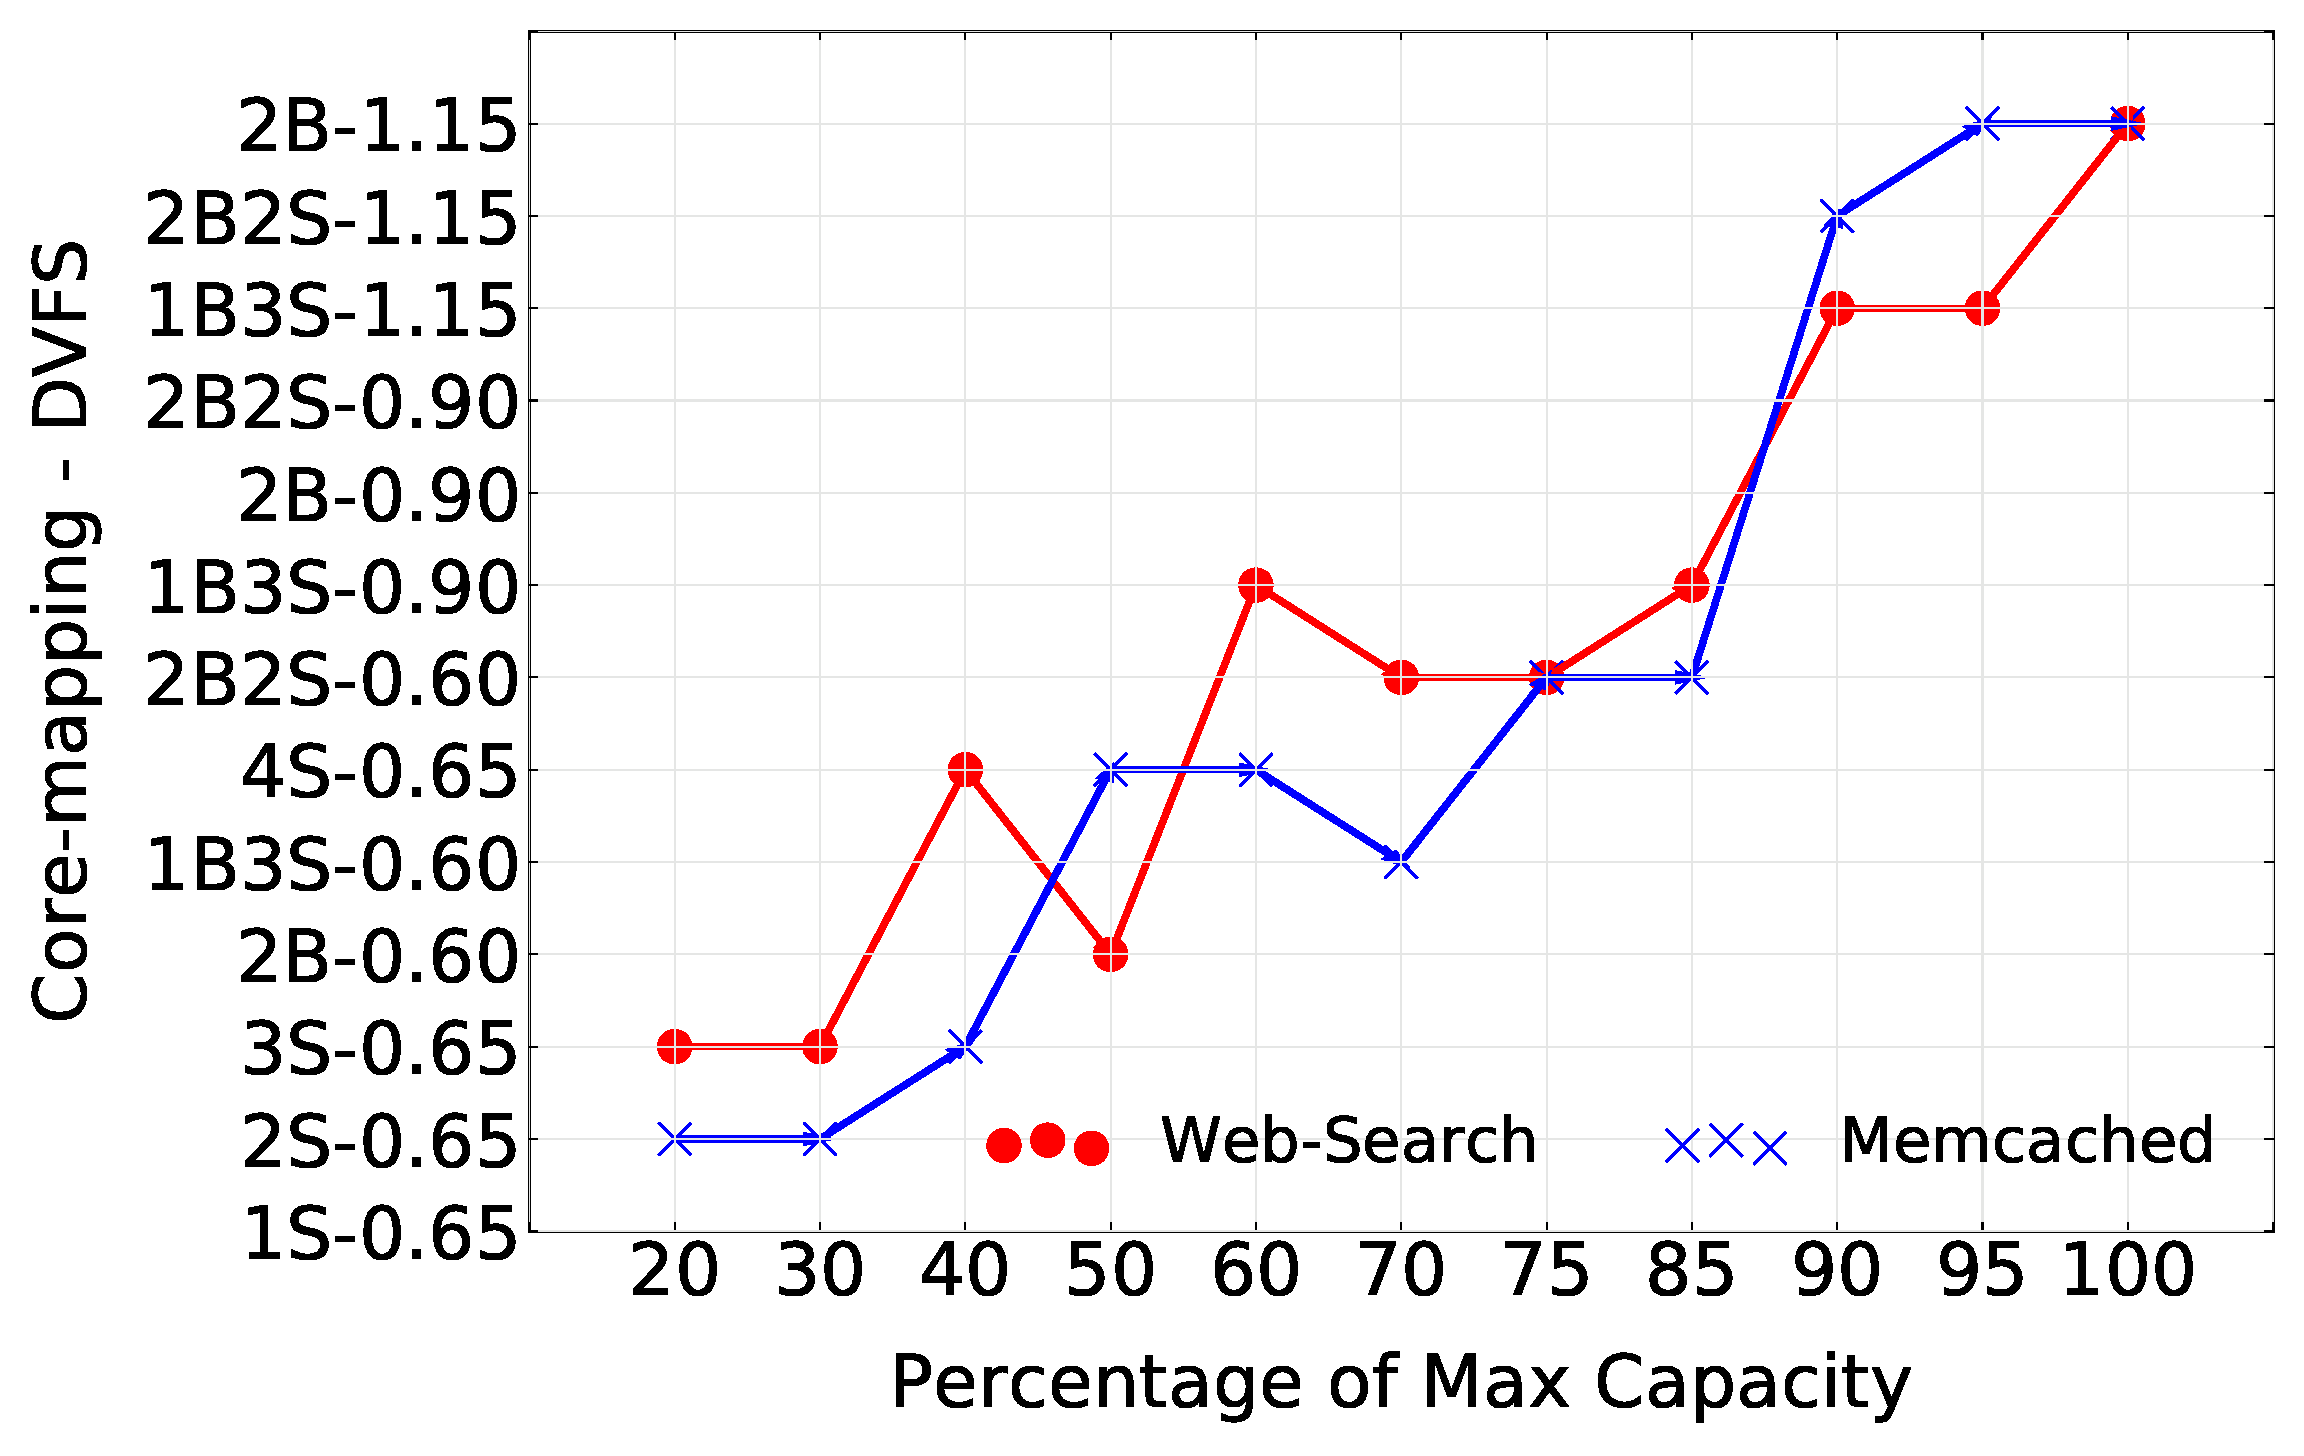
\includegraphics[width=0.9\linewidth]{Chapter4/Figs/state-transition.eps}
  \caption{State Machine}
  \label{fig: state-transition}
\end{subfigure}
    \caption[Throughput per watt of baseline policy vs heterogeneous platform with DVFS]{\captitle{Throughput per watt of baseline policy (BP)~\citep{Petrucci2015Octopus-Man:Computers} vs heterogeneous platform with DVFS (HetCMP).} Throughput per watt of Memcached (\ref{fig: improvements}) and Web-Search (\ref{fig: improvements-websearch}) with BP and HetCMP at different load levels along with their respective state machines (\ref{fig: state-transition})}
\label{fig:octomancomp}
\end{figure}

\noindent running Memcached (Figure~\ref{fig: improvements}) and Web-Search
(Figure~\ref{fig: improvements-websearch}) at different load levels. For each policy,
among the configurations where the QoS is met at each load level, the configuration with
the least power consumption is selected.  The table at the bottom of each subfigure shows
the configuration selected by HetCMP and our baseline policy. In the configurations of the
embedded table, $B$ and $S$ represent big and small cores, respectively. The configuration
space for HetCMP consists of core-mappings (big and small cores) and DVFS combinations for
a heterogeneous platform, whereas the baseline policy consists exclusively of either big
or small cores at the highest DVFS. The configurations available for the baseline policy
are therefore a subset of HetCMP. Experimental details of the ARM platform are given in
Chapter~\ref{chap: infrastructure}.



Figure~\ref{fig:octomancomp} raises two main concerns with current state-of-the-art
heuristic algorithm~\citep{Petrucci2015Octopus-Man:Computers}. First, Figure~\ref{fig:
improvements} demonstrates in periods of low load (less than \SI{60}{\percent} of max
capacity for Memcached), exclusive use of low performance cores at lower DVFS ensures QoS
is met while reducing static-power, thus making it an excellent option to use for periods
of low load. As the load increases, HetCMP transitions from low performance cores to a
best combination of small and big cores at a given DVFS (for instance, 2 big and 2 small
cores -- 2B2S at \SI{0.9}{\giga\hertz} at \SI{89}{\percent} load) to deliver the required
latency.  On the other hand, the baseline policy transitions directly from low performance
cores to high performance cores at highest DVFS to deliver the required latency, thereby
increasing energy consumption by \SI{27.74}{\percent} (mean). In periods of very high load
(more than \SI{90}{\percent} for Memcached), exclusive use of high performance cores at
higher DVFS ensures QoS is met with better energy proportionality.  Similarly results were
observed for Web-Search (Figure~\ref{fig: improvements-websearch}) with up to
\SI{25}{\percent} (mean) energy savings. The state-machine configuration for Memcached and
Web-Search are represented by the blue and red line, respectively, in Figure~\ref{fig:
state-transition}.

In summary, we show that small and big cores are an attractive option for periods of low
load and very high load, respectively, while meeting QoS targets at a much lower cost. On
the other hand, for intermediate loads, which are generally experienced by data centres
during the day~\citep{Vamanan2015TimeTrader:Search}, harnessing HetCMP provides the
opportunity for higher performance at a lower cost.


\paragraph{Exploring workload particularities.} We note that prior
work~\citep{Petrucci2015Octopus-Man:Computers} relies on a general single heuristic to
allocate exclusively big or small cores to workloads. By allowing an arbitrary allocation
mix of big and small cores with DVFS, this kind of heuristic can be sub-optimal across
diverse applications and architectures (evaluation details in Section~\ref{sec:
evaluation-hipster}); that is, a single state-machine management (as used in prior work)
may fail to precisely satisfy the QoS targets given distinct workload characteristics of
diverse applications. To illustrate this point, Figure~\ref{fig: state-transition} shows
two distinct/unique state transition mappings that are optimal (throughput per watt) at
different load capacities for Memcached and Web-Search.

\begin{figure}[t!]
    \centering
    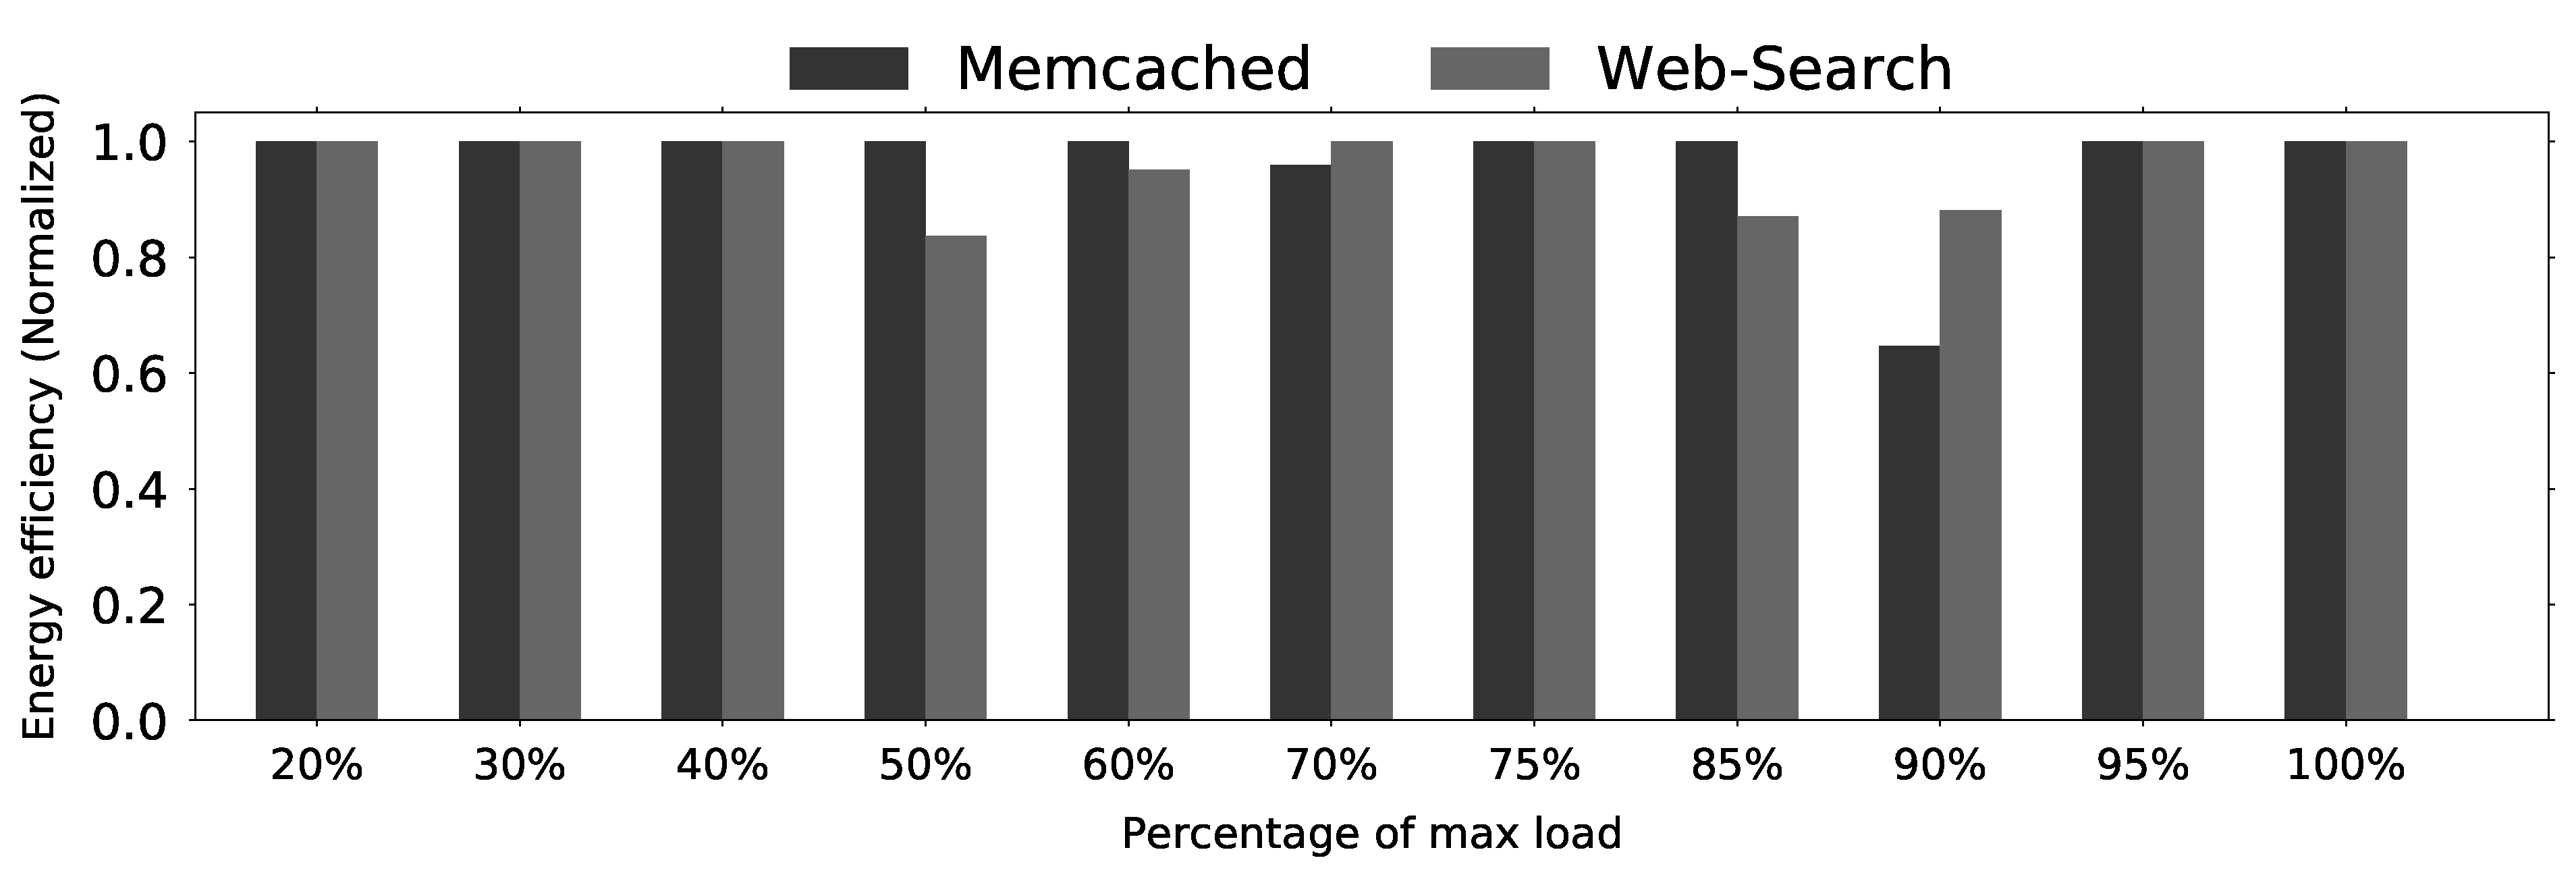
\includegraphics[width=\textwidth]{Chapter4/Figs/config_exchange_new.eps}
    \caption[Energy efficiency of Memcached and Web-Search with state-machines exchanged.]{\captitle{Energy efficiency of Memcached and Web-Search with state-machines exchanged.} Energy efficiency at various load levels for Memcached while meeting QoS, using the state-machine of Web-Search normalised to the state-machine of Memcached (\textit{lower is worse}); converse for Web-Search.}
    \label{fig:config-exchange}
\end{figure}

Figure~\ref{fig:config-exchange} shows the energy efficiency that would be neglected
(ensuring QoS is met at different load levels) when using the state-machine built for
Web-Search but used for the manage the Memcached workload, normalised to the energy
efficiency using the state-machine built exclusively for Memcached; and vice-versa. The
state-machine configuration for Memcached and Web-Search are represented in blue and red
line, respectively, in Figure~\ref{fig: state-transition}.
Figure~\ref{fig:config-exchange} demonstrates that different latency-critical applications
benefit from different state-transition mappings and show improvement in energy efficiency
up to \SI{35}{\percent} for Memcached (at \SI{90}{\percent} load) and up to
\SI{19}{\percent} for Web-Search (at \SI{50}{\percent} load).  For instance, at low loads
and at very high loads both applications use exclusively small cores (low static power) or
big cores (high static power), respectively.  However, for intermediate loads, the
configurations in the state-transition for Web-Search are not present in Memcached and
vice-versa, thus providing minimal to no energy optimisation.

In practical scenarios, each workload has a time-varying load~\citep{Li2014TalesTail} and
a QoS target that needs to be met. As shown in Figure~\ref{fig:octomancomp}
and~\ref{fig:config-exchange}, there exists a unique configuration for each load  that
optimises energy efficiency. Moreover, the time-varying load presented in two forms:
sudden load spikes~\citep{Dean2013TheScale} or gradual load
changes~\citep{Meisner2011PowerServices, Hoelzle2009TheMachinesb}. Both these forms
present a challenge for a heuristic based approach as it jumps across multiple
configurations to meet the QoS target, thereby leading to QoS violations due to rampant
core oscillations.  Also, Kasture \etal~\citep{Kasture2015Rubik} note that
core-transitions are far more costly -- relative to DVFS changes.

There is a need for application agnostic learning approach that can exploit the energy
efficiency benefits of heterogeneous architectures and DVFS features, and can deal with
sudden/gradual load changes across different levels. This is precisely what
\textbf{Hipster} delivers.


\section{Hipster}%Methodology}
\label{sec: methodology-hipster}


\looseness -1 In this section, we introduce \textbf{Hipster}, a hybrid reinforcement
learning (RL) approach coupled with a feedback controller that dynamically allocates
workloads to heterogeneous cores while selecting optimised DVFS settings.  We propose a
variant, called HipsterIn, that is optimised for latency-critical workloads running solo
in the system, adjusting the system configuration to reduce energy consumption. The
HipsterCo variant, which supports collocation of latency-critical and batch workloads, and
focuses on maximising the throughput of the batch workloads. Both variants of Hipster
always ensure that the QoS requirements are met for the latency-critical workload. 

\subsection{Hipster Reinforcement Learning} \label{subsec:learninng}

The RL problem solved by Hipster is formulated as a Markov Decision Process
(MDP)~\citep{Puterman:1994:MDP:528623}. In an MDP, a decision-making process must learn
the best course of action to maximise its total reward over time.  At each discrete
instant, $n$, the process can observe its current \emph{``state''}, $w_n$, and it must
choose an \emph{``action''} $c_n$ from a finite set of alternatives. Depending on the
chosen action and current state (but nothing else), there is an unknown probability
distribution controlling which state, $w_{n+1}$, it enters next and the reward, $\lambda_n$,
that it receives. The problem is to maximise the total discounted reward, given by
$\sum_{n=0}^{\infty} \gamma^n \lambda_n$, where $\gamma$ is the discounting factor. The
discounting factor $\gamma$ should be positive and (slightly) less than one, in order to
reflect a moderate preference for rewards in the near future. 


\nomenclature[a-wn]{$w_n$}{The current \emph{``state''} in MDP refers to load of the
latency-critical workload measured during time interval $t_{n-1}$ to $t_n$}

\nomenclature[a-cn]{$c_n$}{The action chosen from a finite set of alternatives for the
current state, $w_n$, in time interval $t_{n}$ to $t_{n+1}$} 

\nomenclature[a-wn1]{$w_{n+1}$}{The next \emph{``state''} in MDP based on the current
action, $c_n$} 

\nomenclature[g-tdr]{$\sum_{n=0}^{\infty} \gamma^n \lambda_n$}{The aim of MDP is to maximise
this function, total discounted reward} 


\nomenclature[z-MDP]{MDP}{Markov Decision Process}

\nomenclature[g-lambda]{$\lambda_{n}$}{Positive or negative reward in MDP for the chosen action,
$c_n$ is updated at $t_{n+1}$ }

\nomenclature[g-gamma]{$\gamma$}{Discounting factor in MDP}

\nomenclature[g-xi]{$\xi$}{Learning factor in MDP}

The hybrid task management problem solved by Hipster is translated to an MDP as follows.
The state $w_n$ indicates the current load on the latency-critical workload, measured during the (prior) time interval
$t_{n-1}$ to $t_n$.\footnote{Load is Chapter~\ref{chapter: hipster} (only)
refers to load of the latency-critical workload measured in requests per second, or
queries per second, whereas in Chapter~\ref{chap: REPP} it is referred to as IPS.} Hipster quantises the load into buckets.  Specifically the
latency-critical application provides a measurement of the percentage load during the time
interval, in terms of requests per second, queries per second, or similar. The action,
$c_n$, which is chosen by Hipster depending on the state, determines the configuration to
be used in the (next) time interval, $t_n$ to $t_{n+1}$; that is, the combination of cores
and DVFS settings allocated to the latency-critical application.  These settings are used
for the upcoming interval, at the end of which, at time $t_{n+1}$, the reward $\lambda_n$ is
determined depending on the level of QoS relative to the target, given a metric of
optimisation: either the system power consumption (HipsterIn) or the throughput of the
batch workloads (HipsterCo). A precise definition of the calculation of the reward is
given in Section~\ref{subsec: rewardcalculation}.


RL is a type of unsupervised machine learning with a focus on online
learning~\citep{Mnih2015Human-levelLearning}. It solves an MDP by maintaining a table of
values, $R(w,c)$, indexed on the possible states $w\in W$ and possible actions $c\in C$.
The entry $R(w,c)$ estimates the total discounted reward that will be received, starting
from state $w$, if the decision-making process starts by choosing next action $c$.
Assuming that the \textbf{lookup table}, $R(w,c)$ has close to correct values, then, if
the current state is $w_n$, the best action $c_n$ is the one that gives the largest total
discounted reward; i.e. $c_n = \arg\max_c R(w_n, c)$.  The process chooses this value of
$c_n$, then it updates $R(w_n, c_n)$ using a particular formula based on the old and new
states, $w_n$ and $w_{n+1}$, and the reward $\lambda_n$.\footnote{The update of
$R(w_n,c_n)$ is on line~17 of Algorithm~\ref{pseudo:reward}.} A classic problem in RL is
known as the \textit{exploitation--exploration dilemma}, which captures the need not only
to exploit the best solution identified so far, but also to fully explore alternatives,
which may or may not be better.  

\nomenclature[a-rwc]{$R(w,c)$}{A lookup table of rewards for state $w$ and action $c$}

\nomenclature[a-ba]{$c_n = \arg\max_c R(w_n, c)$}{The action with the highest reward,
$c_n$ among the possible set of actions, $c$, for the current state, $w_n$}


Hipster uses a hybrid RL approach~\citep{TesauroAAllocation}, which combines reinforcement
learning with a heuristic, to be used while the algorithm is still learning the optimal
behaviour. For Hipster, the heuristic improves QoS at the beginning of the execution and
it is also re-used after a change in the characteristics of the problem, e.g.\ the mix of
batch workloads. A hybrid RL~\citep{TesauroAAllocation} has the potential to outperform
pure RL schemes~\citep{2007IBMReports,Tesauro2005OnlineLearning.} that only deal with the
exploitation--exploration dilemma (e.g.\ Q-learning), for several reasons: 

\begin{itemize}

    \looseness -1 \item[{\small \circled{1}}] During the learning phase, online
        unsupervised learning without a heuristic generates random decisions, which would
        produce an unacceptable number of QoS violations.

\looseness -1 \item[{\small \circled{2}}] As the complexity of the problem increases, in
    terms of workloads, number of cores, DVFS settings, and so on, it may take longer to
        learn the table $R$. In contrast, a hybrid RL can find acceptable solutions even
        during the learning phase.

\looseness -1 \item[{\small \circled{3}}] The exploration feature of many RL approaches is
    necessary to capture a global maximum, but it may cause extra QoS violations.  Using a
        heuristic in the learning phase can reduce the need to explore configurations that
        clearly violate QoS.

\end{itemize}


\subsection{Hipster Design}
\label{subsec: design}

\begin{figure}[htbp]
    \centering
    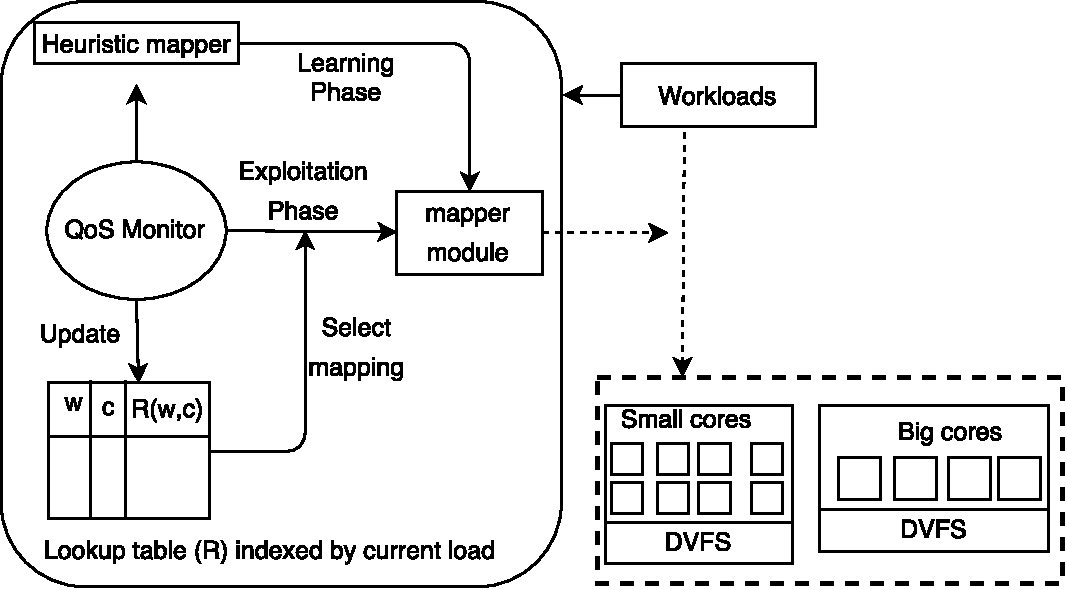
\includegraphics[scale=0.6]{Chapter4/Figs/RIL-Vinson-nocloud-new.pdf}
    \caption{High-level view of Hipster runtime system} 
    \label{fig:hipsteroverview}
\end{figure}

Figure~\ref{fig:hipsteroverview} shows a high-level view of Hipster. Hipster includes a
QoS Monitor, a heuristic mapper (used in the learning phase), an Exploitation Phase, and a
Mapper Module (used in both learning and exploitation phase). Given a QoS target, an
incoming load, and a metric to optimise for, Hipster learns the most adequate core
configuration and DVFS settings by managing a lookup table that is used to map the
workloads to the available hardware resources.

\paragraph*{QoS Monitor.} The QoS Monitor is responsible for periodically collecting the
performance statistics from the latency-critical and batch workloads. For the
latency-critical workload, Hipster gathers the appropriate application-level QoS
metrics such as throughput (RPS or QPS) and latency (query tail latency). It also reads
the current load on the latency-critical workload and quantises this value into discrete
buckets between 0 and $T-1$, for (some) small value $T$. HipsterCo uses a profiling tool
to measure the throughput of the batch workloads, using per core hardware performance
counters, such as CPU utilisation, cache-misses and IPS.

\paragraph*{Learning and exploitation phases.} The data collected by the QoS monitor is used
to make the thread-to-core mapping decisions. In the learning phase, Hipster uses a
feedback control loop based on heuristics to map the latency-critical workload to
resources. Following the intuition from Section~\ref{sec:Motivation}, when load is low,
the mapper executes the latency-critical workload on small cores at lower DVFS states, and
when load is high, it uses a combination of big and small cores at higher DVFS.  Hipster
also begins populating the lookup table so that each entry approximates the corresponding
total discounted reward.  Specifically, Hipster uses the reward mechanism
(Section~\ref{subsec: rewardcalculation}) to prefer core configurations that minimise
system energy consumption or maximise batch workload throughput, while ensuring as well as
possible that at least \SI{95}{\percent} QoS guarantee is achieved~\citep{Horvath2007DynamicControl}.

In the exploitation phase, Hipster uses the lookup table to select the core mapping and
DVFS settings, based on the load. It also continues to update the values in the lookup
table, in order to continue to improve the mapping decisions. At runtime, Hipster
determines when to dynamically switch between the learning and exploitation phases, based
on a prefixed time quantum. At deployment stage, we ensure that the bucket size for each
workload gives at least \SI{95}{\percent} QoS guarantee~\citep{Li2014TalesTail} with minimal energy
consumption.

\subsection{Heuristic Mapper (Learning Phase)}
\label{subsec: hybrid}

The heuristic mapper is a state machine with a feedback control loop. The current state
identifies the core configuration: the DVFS settings and number and type of cores to use
for the latency-critical workload.\footnote{State machines and Markov Decision Processes
use ``state'' with different meanings. In Section~\ref{subsec: hybrid} (only), ``state''
refers to the core configuration, elsewhere it is the load.} The choice of available
states depends on the platform; that is, the total number and types of cores, and the DVFS
settings. There is a predefined ordering of the states, approximately from highest to
lowest power efficiency. This ordering is determined by measuring the power and
performance of each state using a stress microbenchmark consisting of mathematical
operations without memory accesses.

Whenever QoS is close to being violated, the state machine transitions into the
next-higher power state. The QoS is quantified using the currently measured tail latency
at the \ninefive or \ninenine percentile, denoted $QoS$\textsubscript{curr}. The target tail latency
is denoted by $QoS$\textsubscript{target}. The state machine transitions to the
next-higher state whenever the time interval ends in the so-called \emph{danger zone}
defined by:

\begin{equation*}
\label{eq:Death-zone}
QoS_{\mathit{curr}} > QoS_{\mathit{target}} \times QoS_{\mathit{D}}
\end{equation*}


\nomenclature[a-qoscurr]{$QoS_{\mathit{curr}}$}{Currently measured tail latency at the \ninefive or \ninenine percentile for the latency-critical workload}
\nomenclature[a-qostarget]{$QoS_{\mathit{target}}$}{The target tail latency for the latency-critical workload}
\nomenclature[a-qosD]{$QoS_{\mathit{D}}$}{QoS as a factor of a co-efficient between 0 and 1}
\nomenclature[a-qosS]{$QoS_{\mathit{S}}$}{QoS as a factor of a co-efficient between 0 and $QoS_{\mathit{D}}$}

where $QoS_\mathit{D}$ is a parameter between 0 and 1 that defines the size of the danger
zone. Whether such a state transition improves or degrades performance and whether it
actually increases or decreases power depends on the characteristics of the platform and
the particular workloads. The state machine may have to make several consecutive state
transitions until the QoS is met.

In contrast, whenever the QoS is far from being violated, the state machine transitions
into the next-lower power state. This happens whenever the time interval ends in the
so-called \emph{safe zone} defined by:

\begin{equation*}
\label{eq:Safe-zone}
QoS_{\mathit{curr}} < QoS_{\mathit{target}} \times QoS_{\mathit{S}}
\end{equation*}

where $QoS_\mathit{S}$ is a parameter between 0 and $QoS_\mathit{D}$ that defines the size
of the safe zone. The values of $QoS_\mathit{D}$ and $QoS_\mathit{S}$ are determined to
avoid oscillations between adjacent states.  In particular, $QoS_\mathit{D}$ is
empirically computed in the same way as for
Octopus-Man~\citep{Petrucci2015Octopus-Man:Computers,Horvath2007DynamicControl}.

The heuristic proposed by Octopus-Man is attractive because of its simplicity but it can
be sub-optimal (see Section~\ref{sec:Motivation}, Figure~\ref{fig: state-transition})
because there is no common static ordering of configuration states that works for all
workloads. Moreover, in practice, the state machine may respond slowly to rapid changes in
load. Nevertheless, we found that such a state machine heuristic is suitable to accelerate
the learning phase of the RL algorithm by exploring viable core configurations to quickly
populate reasonable values into the lookup table.

%Algorithm 1: Reward mechanism
\begin{algorithm}[t]
  \caption{Reward mechanism}
  \label{pseudo:reward}
  \begin{algorithmic}[1]
    \Statex \Comment{\emph{Determine reward ${\lambda}_n$ based on interval $t_n\dots t_{n+1}$}}
    
    \State Let $QoS\textsubscript{target}$ be the target QoS of the interactive workload.
    \State $QoS\textsubscript{curr}$ = $QoSMonitorLatency$
    \State $Power$ = $QoSMonitorPower$
    \State $QoS\textsubscript{reward}$ = $QoS\textsubscript{curr} / QoS\textsubscript{target} $ 
    \State $Power\textsubscript{reward} = TDP / Power $ \Comment{\emph{TDP (thermal design power)}}
    \If{$QoS\textsubscript{curr} < QoS\textsubscript{target}\times QoS\textsubscript{D}$}
     \State $\lambda_n = QoS\textsubscript{reward} + 1$
    \ElsIf{$QoS\textsubscript{curr} < QoS\textsubscript{target}$}
    \State $\lambda_n = QoS\textsubscript{reward} + 1 - Random(0,1)$ 
    \Else
    \State $\lambda_n = -QoS\textsubscript{reward} - 1$
    \EndIf
    \If{there exist batch jobs}
      \vspace{2mm}
    \State $\lambda_n = \lambda_n + \frac{B\textsubscript{IPS}+S\textsubscript{IPS}}{maxIPS(B) + maxIPS(S)}$
    \Else
	\State $\lambda_n = \lambda_n + Power\textsubscript{reward}$
    \EndIf
    \State \emph{$\mathrm{\mathbf{if}}$ $\nexists$ $R(w_n, c_n)$~$\mathrm{\mathbf{then}}$~$R(w_n, c_n) = 0$}
    \vspace{2mm} 
    \State $R(w_n,c_n) = R(w_n,c_n) + \xi\Big(\lambda_n + \gamma\max_{d\in C}R(w_{n+1},d) - R(w_n,c_n)\Big)$
    
  \end{algorithmic}
\end{algorithm}


\subsection{Reward Calculation}
\label{subsec: rewardcalculation}

During both the learning and exploitation phases, the values in the lookup table are
dependent on the reward, which is calculated as defined in Algorithm~\ref{pseudo:reward}.
This reward calculation is invoked after each monitoring interval, and its definition was
determined empirically (more details in Section~\ref{subsec: respstab}). The reward
$\lambda_n$ has three parts: the QoS Reward, Stochastic Reward, and either the Power
Reward (for HipsterIn) or the Throughput Reward (for HipsterCo):

\paragraph*{QoS Reward.} The ratio of the measured QoS to the QoS target is known as
$QoS_\mathit{reward}$.  If this value is less than one, then the QoS target has been met,
and it quantifies how quick the response was as the \textbf{QoS earliness}. In this case,
line~7 or~9 applies a positive reward that prefers configurations that approach the QoS
target, which acts as a heuristic to reduce energy consumption or improve batch workload
throughput.  If $QoS_\mathit{reward}$ is greater than one, then the QoS target has
\emph{not} been met, and it determines how intense the violation was as the \textbf{QoS
tardiness}. In this case, line~10 applies a negative QoS reward. 

\nomenclature[a-qosr]{$QoS_{\mathit{reward}}$}{The ratio of $QoS_{\mathit{current}}$ to $QoS_{\mathit{target}}$}


\paragraph*{Stochastic Reward.} When the QoS is below the target, as defined in
Section~\ref{subsec: hybrid}, but still over the danger zone, then a stochastic penalty is
applied (line~9 of Algorithm~\ref{pseudo:reward}). The stochastic penalty offers the
possibility to continue to explore the configuration, but with a smaller probability. In
future, other external influences for the latency-critical workload like noise, contention
on shared resources, pending queue lengths, etc., may cause a QoS violation.



\nomenclature[z-tdp]{TDP}{Thermal Design Power}

\nomenclature[a-powerr]{$Power_{\mathit{reward}}$}{The ratio of $TDP$ to $Power$}

\looseness -1  \paragraph*{Throughput Reward (HipsterCo).} Line~13 of
Algorithm~\ref{pseudo:reward} calculates the Throughput Reward, which is approximately
proportional to the total throughput of the batch workloads. Since HipsterCo does not
require modifications to the batch workloads, it is only possible to measure their
throughput in a generic way using performance counters. Specifically, the throughput is
quantified in terms of IPS. The parameters $B\textsubscript{IPS}$ and
$S\textsubscript{IPS}$ measure the total IPS of the big and small clusters running batch
workloads, respectively. The denominator is constant given by the sum of $maxIPS(B)$ and
$maxIPS(S)$, which measure the maximum IPS, at highest DVFS, for the big and small cores
respectively. Platform specific details are given in Chapter~\ref{chap:
infrastructure}.%Section~\ref{subsec: experimental setup}.  

\paragraph*{Power Reward (HipsterIn).} The ratio of the thermal design power (TDP) to the
measured system power consumption is known as $Power_{\mathit{reward}}$ as shown in
line~15. A smaller value of this term means that the system power consumption was lower,
and it increases the reward. 

\vspace{1.5mm}

Once the reward $\lambda_n$ has been calculated, line~17 updates the value of $R(w_n,
c_n)$ in the lookup table, and this is done in the same way during both the learning and
exploitation phases. This update is controlled using two scalar parameters, both between
zero and one: the learning rate, $\xi$, and, the discounting factor, $\gamma$.

\looseness -1 \paragraph*{Learning Factor, $\xi$.} The $\xi$ coefficient in line~17 of
Algorithm~\ref{pseudo:reward} is the learning factor, which controls the rate at which the
values in the lookup table $R(w,c)$ are updated. A large value of $\xi$ close to one means
that the algorithm learns quickly, favouring recent experience, but increasing
susceptibility to noise. In contrast, a small value of $\xi$ means that the algorithm
learns slowly. In our experiments we used $\xi=0.6$. 

\paragraph*{Discounting Factor, $\gamma$.} The $\gamma$ coefficient in line~17 of
Algorithm~\ref{pseudo:reward} is the discounting factor, which quantifies the preference
for short-term rewards~\citep{Suton.R.S1998ReinforcementIntroduction}. Setting $\gamma=0$
means that the algorithm only relies on immediate short-term rewards. To allow a
balance between short-term and future rewards, we set $\gamma=0.9$ (empirically
determined). In other words, this methodology allows the optimization problem to also
take into account future rewards.



% Algorithm 2: Exploitation phase
\begin{algorithm}[tb]
  \caption{Exploitation Phase}
  \label{pseudo:callreward}
  \begin{algorithmic}[1]
    \State Let $X$ be threshold on QoS guarantee to re-enter learning phase
    \State Let $w_n$ be observed load for interval $t_{n-1}\dots t_n$
    \State Let $c_n$ be configuration for interval $t_n \dots t_{n+1}$
    %\State Let $R(w,c) = 0$ for all $w$, $c$
    \State Let $n = 0$
    \Repeat 

    \Statex \Comment{\emph{At time $t_n$, choose configuration for $t_n$ to $t_{n+1}$}}
    \State Let $c_n = max_{d\in C}R(w_n,d)$	

    \If{there exist batch jobs}
		\State Allocate remaining cores to batch jobs
    	\If{latency-critical jobs on a single core type}
        \State Set highest DVFS for other core type
        \EndIf
     \Else
     	\State Set lowest DVFS for remaining cores     
     \EndIf

     	\State Sleep until $t_{n+1}$  \Comment{\emph{Run for interval $t_n$ to $t_{n+1}$}}
        \State Let $w_{n+1}$ be the quantised load from the latency-critical workload
        \State Call Algorithm~\ref{pseudo:reward} \Comment{\emph{Algorithm~\ref{pseudo:reward} updates $R(w_n,c_n)$}}
    \State $n = n+1$
    
    \State {\textbf{if} $QoS Guarantee \leq X$ \textbf{then} Learning phase}
    \Until{Terminated}
  \end{algorithmic}
\end{algorithm}


\subsection{Exploitation Phase}
\label{subsec: exploitation}

The exploitation phase of Hipster is defined by Algorithm~\ref{pseudo:callreward}. Line~6
determines the configuration, $c_n$, with the highest estimated total discounted reward.
Lines~7 to~12 apply the configuration by mapping the workloads to the resources, as
described below, depending on the specific variant of Hipster (HipsterIn or HipsterCo).
Line~13 runs the workload for the next time interval, and line~15 calls
Algorithm~\ref{pseudo:reward} to update the lookup table, based on the metrics obtained by
the QoS Monitor during the time interval. Line~17 re-enters the learning phase when
necessary.  The mapping of workloads to resources is as follows:

%Need to describe Line~7

\paragraph*{Reward Mechanism for HipsterIn.} To minimise power consumption while meeting
the QoS target for latency-critical workloads, the configuration with the highest reward
is selected and then DVFS setting for the remaining cores is set to the lowest value
(Lines~11 to~12 of Algorithm~\ref{pseudo:callreward}).

\paragraph*{Reward Mechanism for HipsterCo.} Corroborating the findings of prior
work~\citep{Lo2015Heracles}, we observed that collocating both latency-critical and batch
workloads degrades QoS at higher loads due to shared resource contention. If the reward
mechanism were not aware of such collocations, it may make decisions that violate QoS for
the latency-critical workload and/or reduce the throughput of the batch workloads.  As a
precursor to this condition, we introduce the following mechanisms. First, to maximise the
throughput of the throughput-oriented workloads while meeting QoS targets, all of the
unused cores are allocated to the batch workloads (lines~7 to~8 in
Algorithm~\ref{pseudo:callreward}). Second, in case the latency-critical job is allocated
exclusively to a given core type, the other core type is set to the highest DVFS to
accelerate the batch workloads (lines~9 to~12 in Algorithm~\ref{pseudo:callreward}). For
instance, on a two-socket/cluster system with two cores per socket/cluster, if the
latency-critical workload is running on two small cores, the big cores are allocated to
the batch workloads at the highest DVFS. 

\subsection{Responsiveness and Stability}
\label{subsec: respstab}

\looseness -1 To ensure that QoS is met for latency-critical workloads, the scheduling policy must
quickly respond to fluctuations in load and latency, either due to changes in core
mapping, DVFS or any external influence. Therefore, the responsiveness and stability of
Hipster is determined by {\small {\circled{1}}} the computation latency in migrating cores and setting DVFS.
{\small {\circled{2}}} the reaction time of QoS between migrating an application from current mapping to
future mapping, and {\small {\circled{3}}} the granularity of monitoring for the latency-critical workload's
QoS. 

The computational latency for changes in core mapping and DVFS are
negligible~\citep{Cong2012Energy-efficientArchitectures, Leverich2009PowerGating, Madan2011AProcessorsb}.
The default monitoring interval for Memcached and Web-Search is one second. Based on the
aforementioned overheads, we determine the  sampling interval as a sum of the monitoring
interval for the latency-critical application, and the overhead to switch the core mapping
and DVFS.


\subsection{Hipster Implementation}
\label{subsec: implementation}

Hipster is implemented in user space, and it uses minimal hardware support exposed by
Linux. It consists of the QoS Monitor and Mapper Module, together with a lookup table, as
shown in Figure~\ref{fig:hipsteroverview}. 

\looseness -1 \paragraph{QoS Monitor.} Hipster uses a separate process to read the power measurements
using native energy meters, at the sampling interval of the application. In addition to
measuring energy, the QoS Monitor also gathers runtime statistics for the query/request
latency of the latency-critical workload, using a logfile interface. In the case of
HipsterCo, the  batch workload aggregate IPS per core are measured using the performance
monitoring tool, \textsf{perf}~\citep{2016Perf:Counters}, specifically using the
\textit{perf\_event}
\textsf{instructions}~\citep{ARMLimitedARMManual,ARMLimitedARMManualb}. Alternatives to
\textsf{perf} include the profiling tools~\citep{Ren2010Google-WideCenters,
Kanev:2015:PWC:2749469.2750392} supported by Docker, Kubernetes and
LXC~\citep{Bernstein2014ContainersKubernetes}.  

As discussed in Section~\ref{sec: perfmon thesis}, the \textsf{perf} bug on ARM processors
generates garbage values for all cores whenever any core enters an idle state.  Since
performance statistics are required only necessary for the HipsterCo variant (where batch
workloads are collocated with latency-critical workloads), we overcome this by disabling
the CPUidle. 

\vspace{-2mm}

\looseness -1 \paragraph{Mapper Module.} The workloads are mapped to cores using the Linux
\textsf{sched\_setaffinity} call and DVFS is controlled using \textsf{acpi-cpufreq}. In
addition, Hipster suspends and resumes the batch workloads using the relevant OS signals
({\small \textsf{SIGSTOP}} and {\small \textsf{SIGCONT}} in Linux).

\vspace{-1mm}

\looseness -1 \paragraph{Runtime overhead.} Hipster has a simple algorithm, requiring few control flow
statements and main memory accesses, so its runtime overhead is negligible.  We measured
the execution time overhead (implemented in Python and including I/O) to be $<$ \enspace
\SI{2}{\milli\second}, so triggering Hipster every second, as in our experiments, incurs
an overhead $<$ \enspace \SI{0.2}{\percent}.

\begin{wrapfigure}{r}{0.45\textwidth}
%    \centering
    \vspace{-17mm}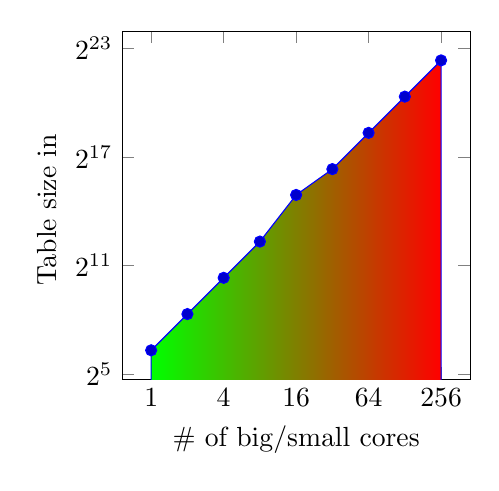
\begin{tikzpicture}
    \begin{axis}[
            xlabel= {\# of big/small cores},
            ylabel= {Table size in $\SI{}{\kilo\byte}$},
            ymode=log,
            log basis y={2},
            enlarge x limits=0.1,
            legend style={
                    at={(0.5,-0.15)},               
                    anchor=north,legend columns=-1
            },
            width=6cm,
            height=6cm,
            point meta={x},
            symbolic x coords={1, 2, 4, 8, 16, 32, 64, 128, 256},
    ]
    \addplot+  [left color=green, right color=red] coordinates {
        (1, 80) (2, 320) (4, 1280) (8, 5120) (16, 30480) (32, 81920) (64, 327680) (128, 1310720) (256, 5242880) } \closedcycle;
    \end{axis}
    \end{tikzpicture}
    \vspace{0mm}
    \caption[Lookup table size in \SI{}{\kilo\byte}]{Lookup table size (log scale) with same number of small and big cores, using 10 different DVFS settings, and bucket size of 100.}
    \vspace{-3mm}
    %\vp{X axis should change "\# of big cores" to "\# of big/small cores"}
    \label{fig:size}
\end{wrapfigure}

\looseness -1 \paragraph{Lookup table.} Each iteration of the RL algorithm accesses and modifies several
entries in the lookup table. To ensure that these operations take negligible time, the
computational complexity to access the table should be at most a few instructions.
Therefore, in the prototype implementation of Hipster, the lookup table was implemented
using a Python dictionary, which uses open addressing to resolve hash collisions, thereby
having a computational complexity of $\mathcal{O}(1)$ irrespective of the
operation~\citep{PattisComplexityHttps://www.ics.uci.edu/pattis/ICS-33/lectures/complexitypython.txt}.

\looseness -1 We observe that the lookup table size can grow quickly (see Figure~\ref{fig:size}) with
the number of big/small cores, DVFS settings, and the number of load buckets. Let us say
there are $B$ big cores and $S$ small cores available, and $B_{f}$ and $S_{f}$ available
DVFS settings for big and small cores, respectively, then the total number of actions in
the table would be $C$($B$+$B_{f}$, $B_{f}$) $\times$ $C$($S$+$S_{f}$, $S_{f}$), where
$C$(x, y) refers to the number of different ways to choose actions ($y$) for out of $x$
distinct elements. This grows in the order of $\mathcal{O}(B^{B_{f}} \times S^{S_{f}})$.



\looseness -1 Figure~\ref{fig:size} shows the unoptimised (or na\"{\i}ve) lookup table size in
\SI{}{\kilo\byte} when the number of big cores is equal to number of small cores ($B$ =
$S$) with 10 DVFS states for big and small cores ($B_{f}$ = $S_{f}$ = 10) with 100 load
buckets ($w$). For instance, 64 cores of each type leads to 40,960,000 combinations (in
contrast to 56 configurations on ARM Juno), which gives a table size of approximately
$\SI{327}{\mega\byte}$ for a whole node.  

To reduce the size of the lookup table in Hipster, we store the configuration and reward
only for the configurations which have been explored so far. The lookup table is still
implemented using a Python dictionary as the complexity is $\mathcal{O}(1)$ irrespective
of the operation. Furthermore, in the exploitation phase, we ensure that each load bucket
($w$) contains \emph{only} the top $K$ (in our case, $K=5$) configurations with highest
discounted maximum rewards. 


\section{Evaluation}
\label{sec: evaluation-hipster}

\begin{figure*}[htbp]
    \hspace{5mm}\begin{subfigure}[t]{0.45\textwidth}
    \centering        
    \begin{overpic}[width=\linewidth]{Chapter4/Figs/static-big-memcached-nolabel.eps}
        \put(40,95) {Memcached}
        \put(-5,15){\rotatebox{90}{Static mapping (all big cores)}}
        
     \end{overpic}
    \caption{Static mapping (all big cores)}
	\label{fig: Memcached-static}
\end{subfigure}%
    \hspace{2mm}\begin{subfigure}[t]{0.45\textwidth}
    \centering
    \begin{overpic}[width=\linewidth]{Chapter4/Figs/static-big-elasticsearch-nolabel.eps}
        \put(40,95) {Web-Search}
    \end{overpic}
    \caption{Static mapping (all big cores)}
	\label{fig:staticelasticsearch}
\end{subfigure}
    \hspace{5mm}\begin{subfigure}[t]{0.45\textwidth}
    \centering
        %\includegraphics
        \begin{overpic}[width=\linewidth]{Chapter4/Figs/octoman-memcached.eps}
            \put(-5,25){\rotatebox{90}{Octopus-Man}}
        \end{overpic}
  	\caption{Octopus-Man}
    \label{fig:octoman Memcached}
\end{subfigure}%
\hspace{2mm}\begin{subfigure}[t]{0.45\textwidth}
    \centering
    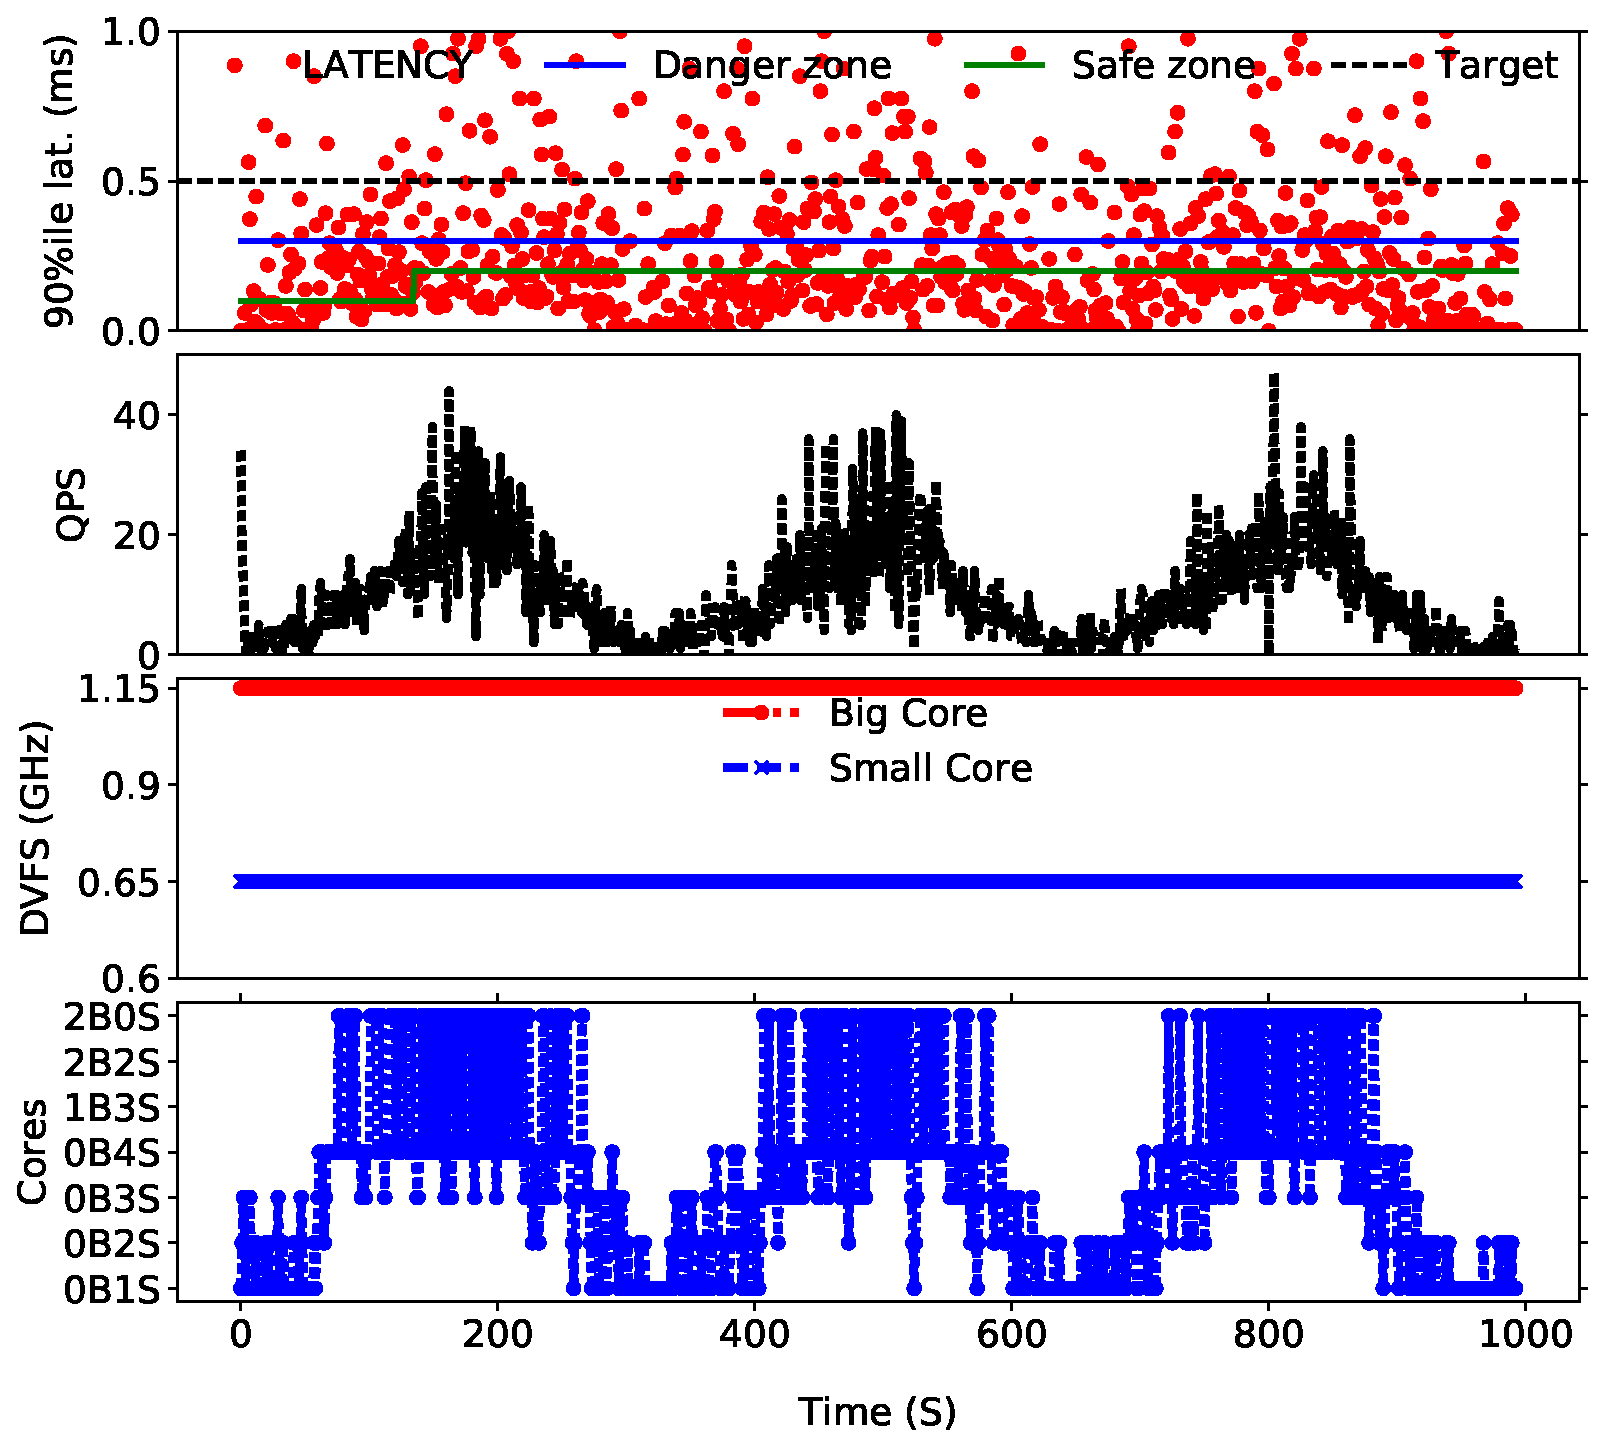
\includegraphics[width=\linewidth]{Chapter4/Figs/octoman-elasticsearch.eps}
  	\caption{Octopus-Man}
    \label{fig:octoman-elasticsearch}
\end{subfigure}
\hspace{5mm}\begin{subfigure}[t]{0.45\textwidth}
    \centering
        %\includegraphics
        \begin{overpic}[width=\linewidth]{Chapter4/Figs/memcached-heursitic.eps}
            \put(-5,15){\rotatebox{90}{Hipster's heuristic mapper}}
        \end{overpic}
    \caption{Hipster's heuristic mapper}
    \label{fig:Memcachedheuristic}
\end{subfigure}%
    \hspace{2mm}\begin{subfigure}[t]{0.45\textwidth}
	\centering
    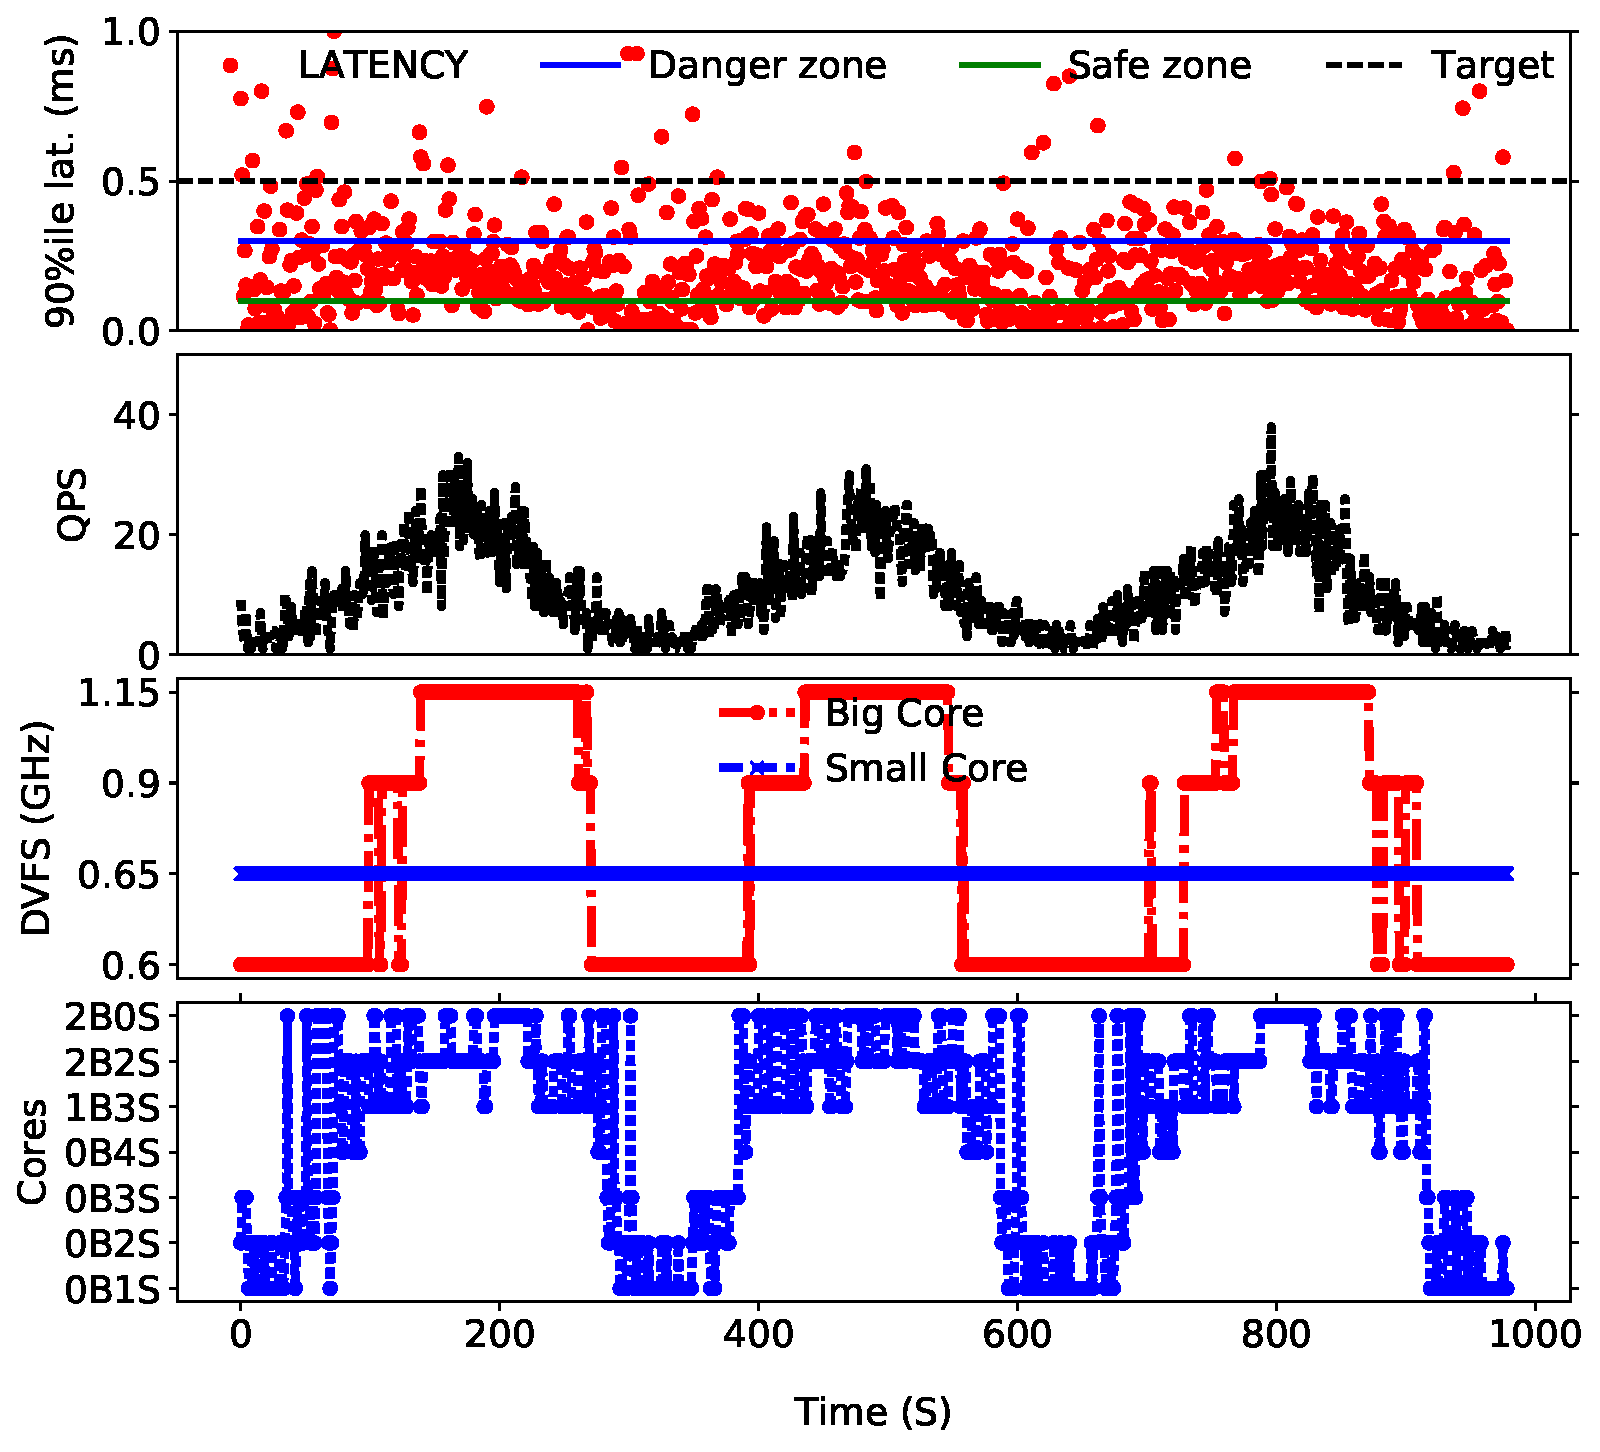
\includegraphics[width=\linewidth]{Chapter4/Figs/ourheuristic-es.eps}
	\caption{Hipster's heuristic mapper}
	\label{fig: ourheuristic-es}
\end{subfigure}
    \caption[Comparision of heuristic policies]{\captitle{Comparison of heuristic policies.} Static mapping (top), Octopus-Man (middle), and Hipster's heuristic policy (bottom). Results are shown for Memcached (left-hand column) and Web-Search (right-hand column) on ARM Juno R1.}
    %Hipster's heuristic policy (right-hand column) with static mapping (left) and Octopus-Man (centre). Results are shown for Memcached (top) and Web-Search (bottom) on ARM Juno R1.}
\label{fig:heuristic}
\end{figure*} 


\subsection{Algorithm Configuration}

In deploying Octopus-Man, we first performed a sweep on the danger and safe thresholds,
and picked the combination of thresholds with the highest QoS guarantee. For HipsterIn, we
set the learning phase to be 500~seconds, except when quantifying the learning time, where
we set it to 200~seconds. In addition, we quantify HipsterIn with changes in application
at runtime, where we run each application for 1500~seconds.



\subsection{HipsterIn Results} 
\label{subsec: results}

This section evaluates the effectiveness of HipsterIn, as a policy for managing a single
interactive workload.  The objective is to minimise system energy consumption while
satisfying QoS.

\subsubsection{Hipster's Heuristic Policy (interactive only)}
\label{subsubsec: heuristic interactive}

\looseness -1 We first evaluate the effectiveness of Hipster's heuristic policy alone, for
mapping interactive workloads. Figure~\ref{fig:heuristic} shows the results for both
workloads: Memcached (left-hand column , subfigures (a), (c) and (e)) and Web-search
(right-hand column, subfigures (b), (d) and (f)). The rows, from top to bottom, correspond
to static mapping, for which the interactive threads are mapped to the two big cores at
highest DVFS of \SI{1.15}{\giga\hertz} ((a) and (b)), Octopus-Man ((c) and (d)) and
Hipster's heuristic policy ((e) and (f)). For each subfigure, from top to bottom, the
first plot presents the tail latency (QoS), with the target marked with a dashed line.
The second plot shows the achieved throughput in RPS (requests per second). The third plot
presents the DVFS of the big and small cores, and the fourth plot represents the choice of
core mapping.

\looseness -1 Comparing the DVFS and core configuration subplots, we observe that
Hipster's heuristic policy is successfully exploring the DVFS settings available on the
Juno platform (bottom plots), and it is exploring all configurations including those that
use both big and small cores at the same time (bottom plots).  In contrast, Octopus-Man
does not adjust the DVFS settings and it uses either the big or small cores, but not both
at once. 

Both Octopus-Man and Hipster's heuristic policy frequently oscillate between consecutive
core configurations.  In the case of Octopus-Man, there are clear oscillations between two
big cores and four small cores, for example between the $600^{th}$ and $800^{th}$ seconds.
Using two big cores satisfies QoS but since it is within the safe zone, Octopus-Man
switches to four small cores, which enters the danger zone, generating an alert provoking
a return to two big cores. Such oscillations between cores in different clusters leads to
severe QoS degradation of up to \SI{20}{\percent}. As expected, the static mapping (all
big cores) has the least number of violations. 

\looseness -1 In summary, although Hipster's heuristic policy alone improves over
Octopus-Man by exploiting a wider search space, it still suffers from an unacceptable
number of QoS violations.

\begin{figure*}[b!]
\begin{minipage}[b]{.48\textwidth}
	\centering
	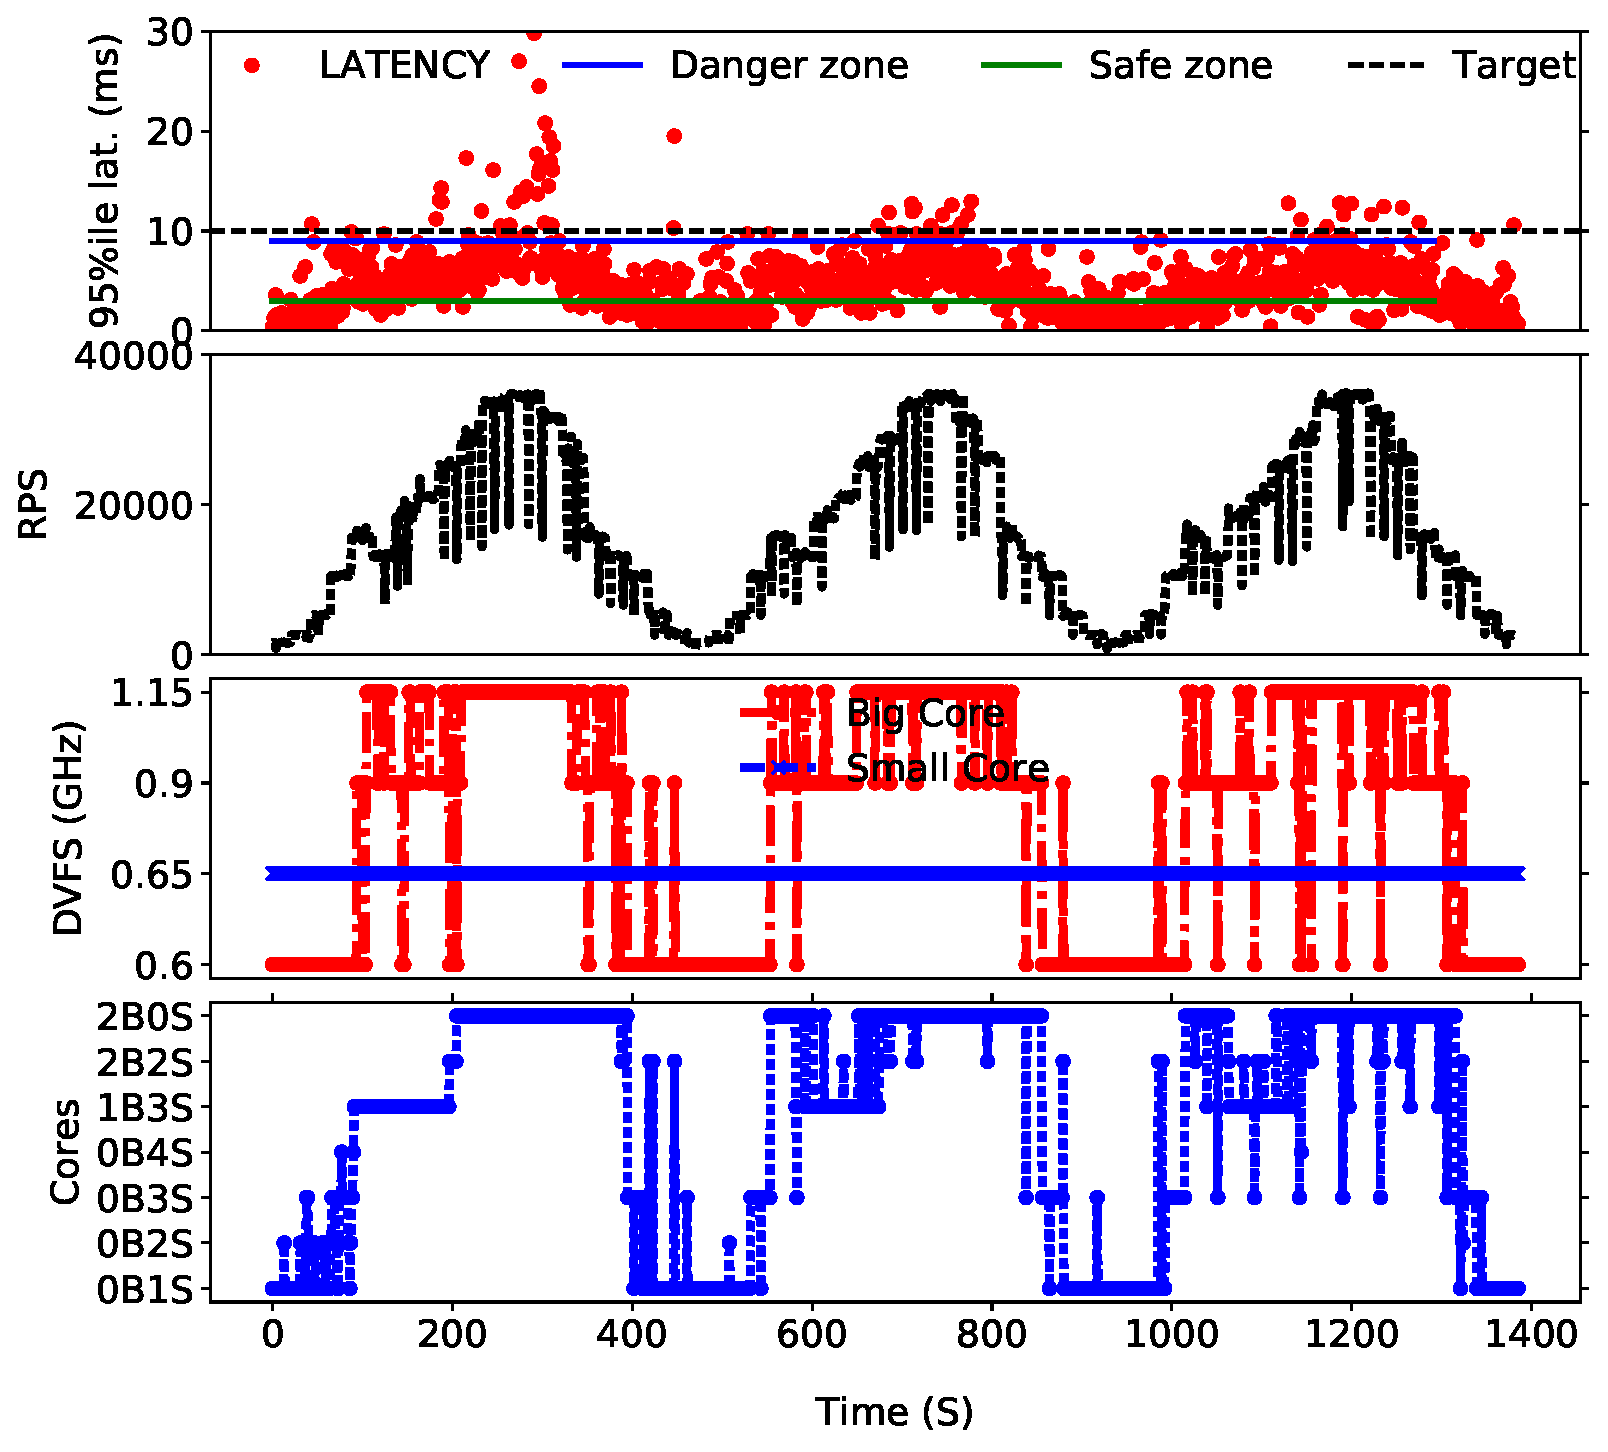
\includegraphics[width=\linewidth]{Chapter4/Figs/hipster-memcached-copy.eps}
    \caption[HipterIn on Memcached]{HipsterIn on Memcached}
    %\caption[HipterIn on Memcached]{HipsterIn on \\ \hspace*{19.5mm} Memcached}
	\label{fig: hipster-memcached} 
\end{minipage}
\hfill
\begin{minipage}[b]{.48\textwidth}
	\centering
	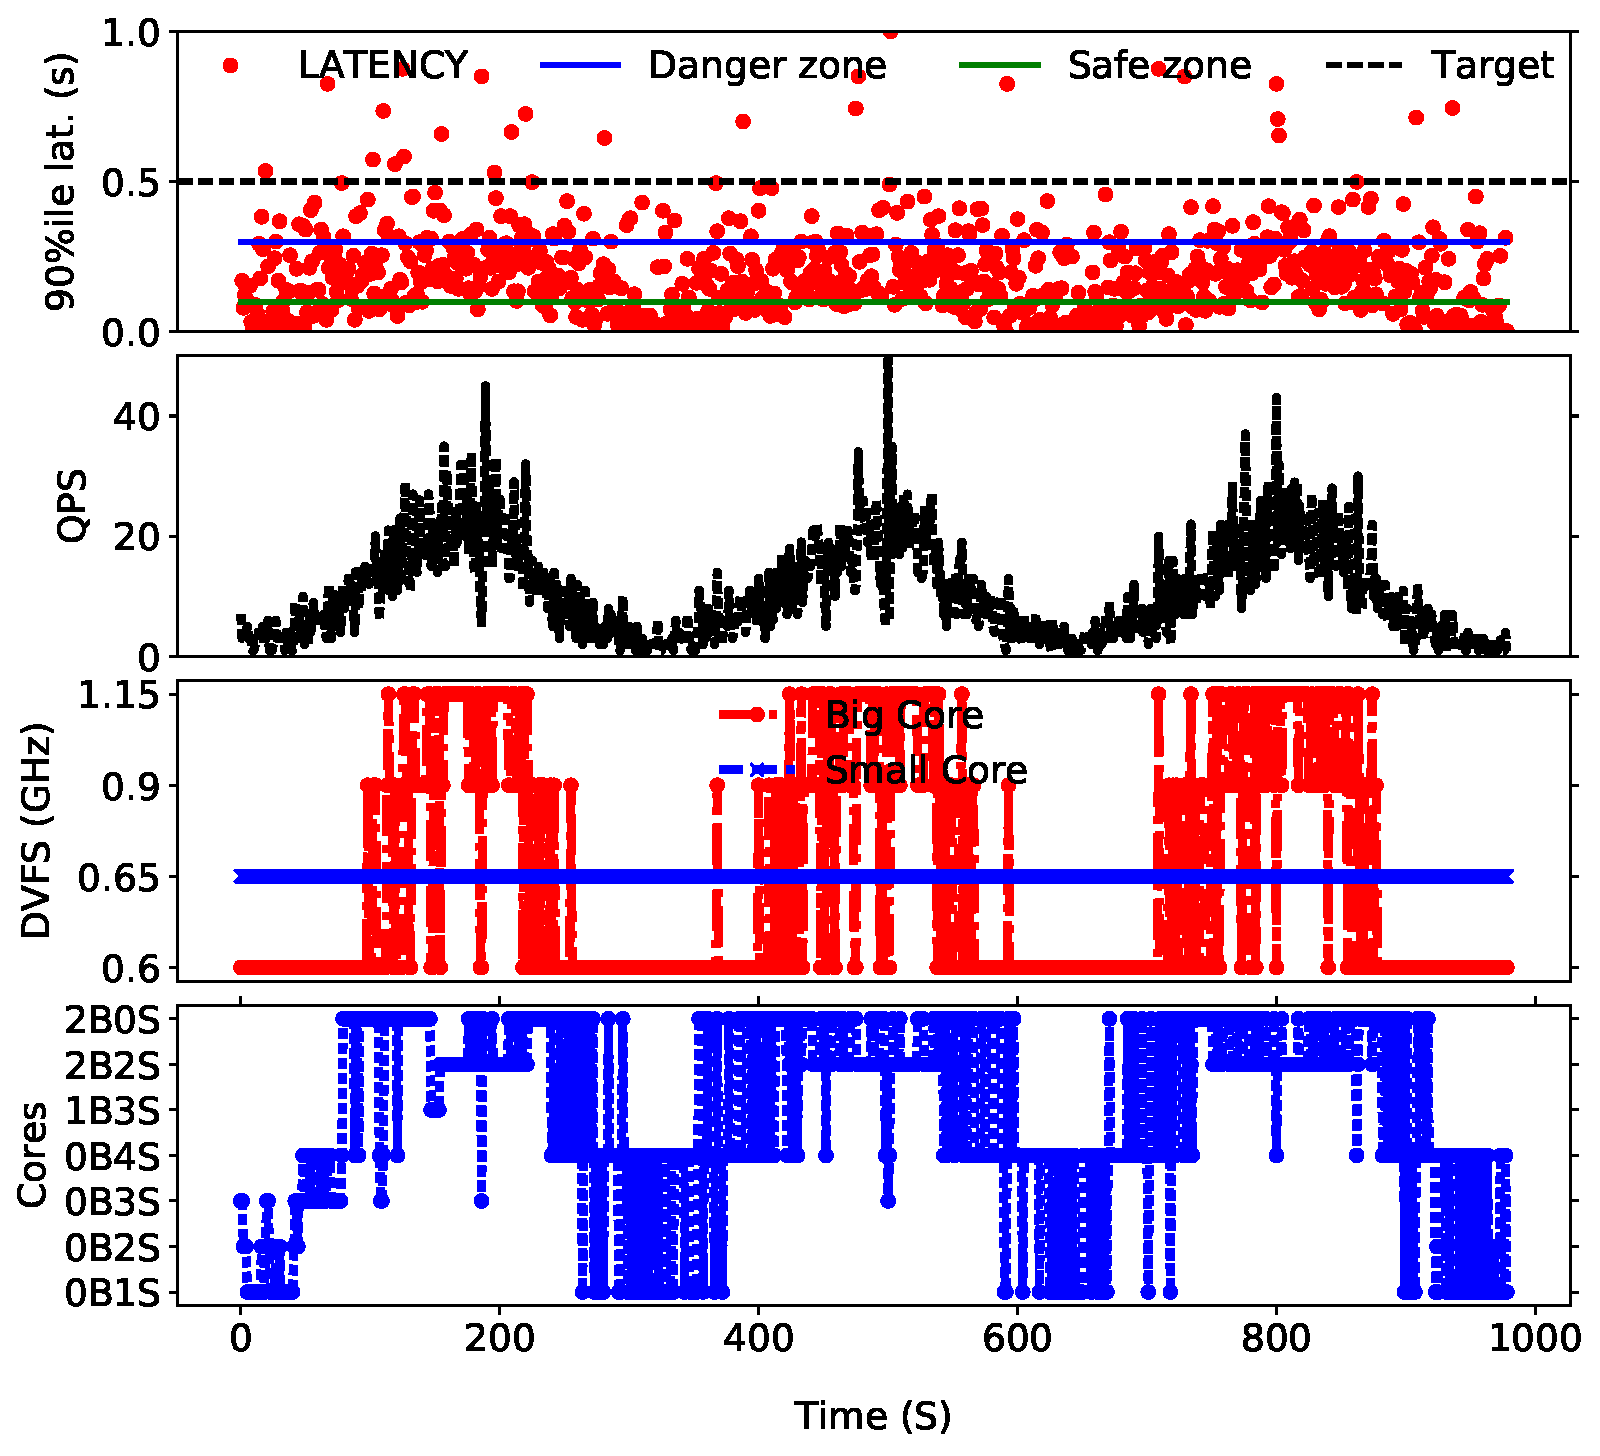
\includegraphics[width=\linewidth]{Chapter4/Figs/ril-elasticsearch.eps}
    \caption[HipsterIn on Web-Search]{HipsterIn on Web-Search}
    %\caption[HipsterIn on Web-Search]{HipsterIn on \\ \hspace*{19.5mm} Web-Search}
	\label{fig: hipster-elasticsearch}
\end{minipage}
\end{figure*}


\subsubsection{HipsterIn: Memcached Results}
\label{subsubsec: memcached results}

Figure~\ref{fig: hipster-memcached} shows the results using HipsterIn for Memcached.
After completing the learning phase, the oscillatory effect between core mappings is
greatly reduced (by \SI{8.3}{\percent}), and overall the QoS guarantee is improved by
\SI{24}{\percent} compared with the learning phase. HipsterIn performs well because it
moves directly to the appropriate core configuration for a given load that satisfies QoS. 

In addition to switching between a combination of different cores, HipsterIn also explores
more fine-grained DVFS adaptations, which has lower overheads (of microseconds) compared
with migrations between cores (order of milliseconds)~\citep{Kasture2015Rubik}.

\subsubsection{HipsterIn: Web-Search Results}
\label{subsubsec: web-search results}

Figure~\ref{fig: hipster-elasticsearch} shows the results using HipsterIn for Web-Search.
In contrast to the heuristic policies (Octopus-Man and Hipster's heuristic), during the
exploitation phase, HipsterIn monitors the QoS and dynamically adjusts the core mapping
and DVFS settings to adapt to load fluctuations. Both Hipster's heuristic and Octopus-Man
perform aggressive changes to core mappings to reduce energy, leading to a negative impact
on QoS. On the other hand, HipsterIn shows a more balanced behaviour, performing
$4.7\times$ fewer task migrations than Octopus-Man for Web-Search, while improving QoS up
to \SI{16}{\percent} and reducing energy consumption by \SI{13.5}{\percent}. 

\subsubsection{\textbf{HipsterIn: Swapping applications}}
\label{subsubsec: swap apps}

%We also evaluate the effectiveness of HipsterIn to adapt to changes in application with
%different characteristics at runtime.

We also evaluate the effectiveness of HipsterIn to adapt to changes in application at
runtime and deliver real-time performance guarantees even for the new incoming
application.

\paragraph*{Web-Search to Memcached} Figure~\ref{fig: hipster-elasticsearch-memcached}
shows the results using HipsterIn when swapping from Web-Search (represented in red) to
Memcached (represented in cyan) after \SI{1500}{\second} of execution. ``NA''
in the last two subplots on $y$-axis represents the period when Web-Search or Memcached are running
exclusively. HipsterIn shows a more balanced behaviour, performing 22\% fewer violations
than learning phase, set at 500-seconds, when running Web-Search. Thereafter, when
swapping Web-Search with Memcached observe that HipsterIn has a far more QoS violations
but quickly adapts to changes in application by learning the lookup table suitable for
Memcached.

\begin{figure*}[htb]
	\centering
    \begin{overpic}[width=\textwidth]{Chapter4/Figs/memcached-websearch.eps}
        \put(2.8,24.5){\tiny NA}
        \put(2.8,9.5){\tiny NA}
    \end{overpic}
	\caption{HipsterIn on Memcached swapping to Web-Search}
	\label{fig: hipster-memcached-websearch} 
\end{figure*}

\paragraph*{Memcached to Web-Search} Figure~\ref{fig: hipster-memcached-websearch} shows
the results using HipsterIn when swapping from Memcached (represented in cyan) to
Web-Search (represented in red) after \SI{1500}{\second} of execution. ``NA''
in the last two subplots on the $y$-axis represents the period when Memcached or Web-Search are running
exclusively.  When application is swapped at runtime from Memcached to Web-Search,
HipsterIn dynamically updates the lookup table to adapt to changes in application
behaviour. For instance, observe at \SI{1500}{\second}, HipsterIn has large number of
violations (by \SI{7.1}{\percent}) but quickly drops after it adapts the lookup table and
the overall QoS guarantee is improved by \SI{38}{\percent}. The QoS guarantee of HipsterIn for Web-Search is 95\%, which is similar to QoS guarantee when running Web-Search from the start (Table~\ref{tab: summarytable-hipster})

\begin{figure*}[htb]
	\centering
    \begin{overpic}[width=\textwidth]{Chapter4/Figs/websearch-memcached.eps}
        \put(2,24.5){\tiny NA}
        \put(2,9.5){\tiny NA}
    \end{overpic}
	\caption{HipsterIn on Web-Search swapping to Memcached}
	\label{fig: hipster-elasticsearch-memcached}
\end{figure*}




\subsubsection{HipsterIn Summary}
\label{subsubsec: summaryresults}

\iffalse
\begin{table*}[t]
\centering
%\ra{1.4}
\setlength{\tabcolsep}{2pt}
    \caption[Summary of HipsterIn for Memcached, and Web-Search]{\captitle{Summary of HipsterIn for Memcached and Web-Search.} A summary of QoS guarantees, tardiness and energy savings}
%\caption{HipsterIn: summary of QoS guarantees, tardiness and energy savings for Memcached and Web-Search.}
\scalebox{1}{
\begin{tabular}{@{}lrrcrrcrr@{}}\toprule
& \multicolumn{2}{c}{$QoS\enspace Guarantee$} & \phantom{abc}& \multicolumn{2}{c}{$QoS\enspace Tardiness$} & \phantom{abc} & \multicolumn{2}{c}{$Energy\enspace Reduction$}\\
\cmidrule{2-3} \cmidrule{5-6} \cmidrule{8-9}
& $Memcached$ & $Web-Search$ && $Memcached$ & $Web-Search$ && $Memcached$ & $Web-Search$ \\ 
\midrule
$Static\enspace$ (all big cores)   & 99.5\% & 99.5\%  && 1.1  & 1.3   && -       & -\\
$Static\enspace$ (all small cores) & 85.8\% & 78.4\%  && 1.4  & 2.0   && 48.0\% & 31.0\%\\
$Hipster's\enspace Heuristic$        & 89.9\% & 95.3\%   && 1.8  & 1.9   && 18.7\%  & 13.6\%\\
$OctopusMan$                   & 92.0\% & 80.0\%  && 2.2  & 2.1   && 17.2\%  & 4.3\%\\
$\textbf{HipsterIn}$             & \textbf{99.4\%} & \textbf{96.5\%} && 1.4  & 2.0 && \textbf{14.3\%}  & \textbf{17.8\%}\\
\bottomrule
\end{tabular}
}
\label{tab: summarytable-hipster}
\end{table*}
\fi

\begin{table*}[t]
\centering
%\ra{1.4}
\setlength{\tabcolsep}{2pt}
\caption[Summary of HipsterIn for Memcached, and Web-Search]{\captitle{Summary of HipsterIn for Memcached (Mem) and Web-Search (Web).} A summary of QoS guarantees, tardiness and energy savings}
%\caption{HipsterIn: summary of QoS guarantees, tardiness and energy savings for Memcached and Web-Search.}
\scalebox{0.95}{
\begin{tabular}{@{}lrrcrrcrr@{}}\toprule
& \multicolumn{2}{c}{$QoS\enspace Guarantee$} & \phantom{abc}& \multicolumn{2}{c}{$QoS\enspace Tardiness$} & \phantom{abc} & \multicolumn{2}{c}{$Energy\enspace Reduction$}\\
\cmidrule{2-3} \cmidrule{5-6} \cmidrule{8-9}
& $Mem$ & $Web$ && $Mem$ & $Web$ && $Mem$ & $Web$ \\ 
\midrule
$Static\enspace$ (all big cores)   & 99.5\% & 99.5\%  && 1.1  & 1.3   && -       & -\\
$Static\enspace$ (all small cores) & 85.8\% & 78.4\%  && 1.4  & 2.0   && 48.0\% & 31.0\%\\
$Hipster's\enspace Heuristic$        & 89.9\% & 95.3\%   && 1.8  & 1.9   && 18.7\%  & 13.6\%\\
$OctopusMan$                   & 92.0\% & 80.0\%  && 2.2  & 2.1   && 17.2\%  & 4.3\%\\
$\textbf{HipsterIn}$             & \textbf{99.4\%} & \textbf{96.5\%} && 1.4  & 2.0 && \textbf{14.3\%}  & \textbf{17.8\%}\\
\bottomrule
\end{tabular}
}
\label{tab: summarytable-hipster}
\end{table*}


Table~\ref{tab: summarytable-hipster} summarises the QoS guarantee, QoS tardiness and
energy reduction for Memcached and Web-Search for different policies: Static (all big
cores), Static (all small cores), Hipster's heuristic mapper, Octopus-Man and HipsterIn.
We compare the energy consumption of each mapping schema against Static (all big cores).
We quantify the QoS behaviour at each sampling interval by assessing the measured QoS
using two metrics: QoS guarantee and QoS tardiness.\footnote{QoS Tardiness is
$QoS_{\mathit{curr}}$/$QoS_{\mathit{target}}$, using the definitions from
Section~\ref{subsec: rewardcalculation}.} The QoS Guarantee is the percentage of  samples
for which the measured QoS did not violate the target (\SI{100}{\percent}-QoS
violations\%). The QoS tardiness in the table is the average (mean) of the QoS tardiness,
including only the samples that violated the QoS target.

As shown in Table~\ref{tab: summarytable-hipster}, for Web-Search and Memcached, static
(all small cores) cannot meet the required QoS. On the one hand, the heuristic policies
reduce energy marginally, but violate QoS due to excessive core migrations. On the other
hand, HipsterIn meets QoS at \SI{99.4}{\percent} and \SI{96.4}{\percent} for Memcached and
Web-Search, while having energy savings of \SI{14.3}{\percent} and \SI{17.8}{\percent},
respectively.



\subsubsection{HipsterIn Analysis}




\paragraph*{Rapid adaptation to load changes.} Hipster can respond to rapid changes in
load by directly mapping to a configuration that satisfies the QoS.  Figure~\ref{fig:
responsivenesstoloadchange} shows how HipsterIn (during the exploitation phase) and
Octo\-pus-Man respond to changes in load. From top to bottom, we express the input load in
terms of the percentage of maximum load, where it increases from \SI{50}{\percent} to
\SI{100}{\percent} over a period of 175 seconds for Memcached. In the second graph, we
express the \ninefive percentile tail latency as QoS Tardiness. A QoS violation has
occurred if the QoS Tardiness is above 1, otherwise QoS is satisfied.  We find that
Octopus-Man violates QoS due to aggressive core mappings to minimise energy consumption.
By contrast, HipsterIn achieves more stable tail latency even at higher load
(\SI{80}{\percent}). Note that, from \SI{75}{\percent} to \SI{90}{\percent} of the load,
the QoS tardiness (extent of violation) experienced by HipsterIn is $3.7\times$ (mean)
lower than Octopus-Man. 

\begin{figure}[t]
	\centering
	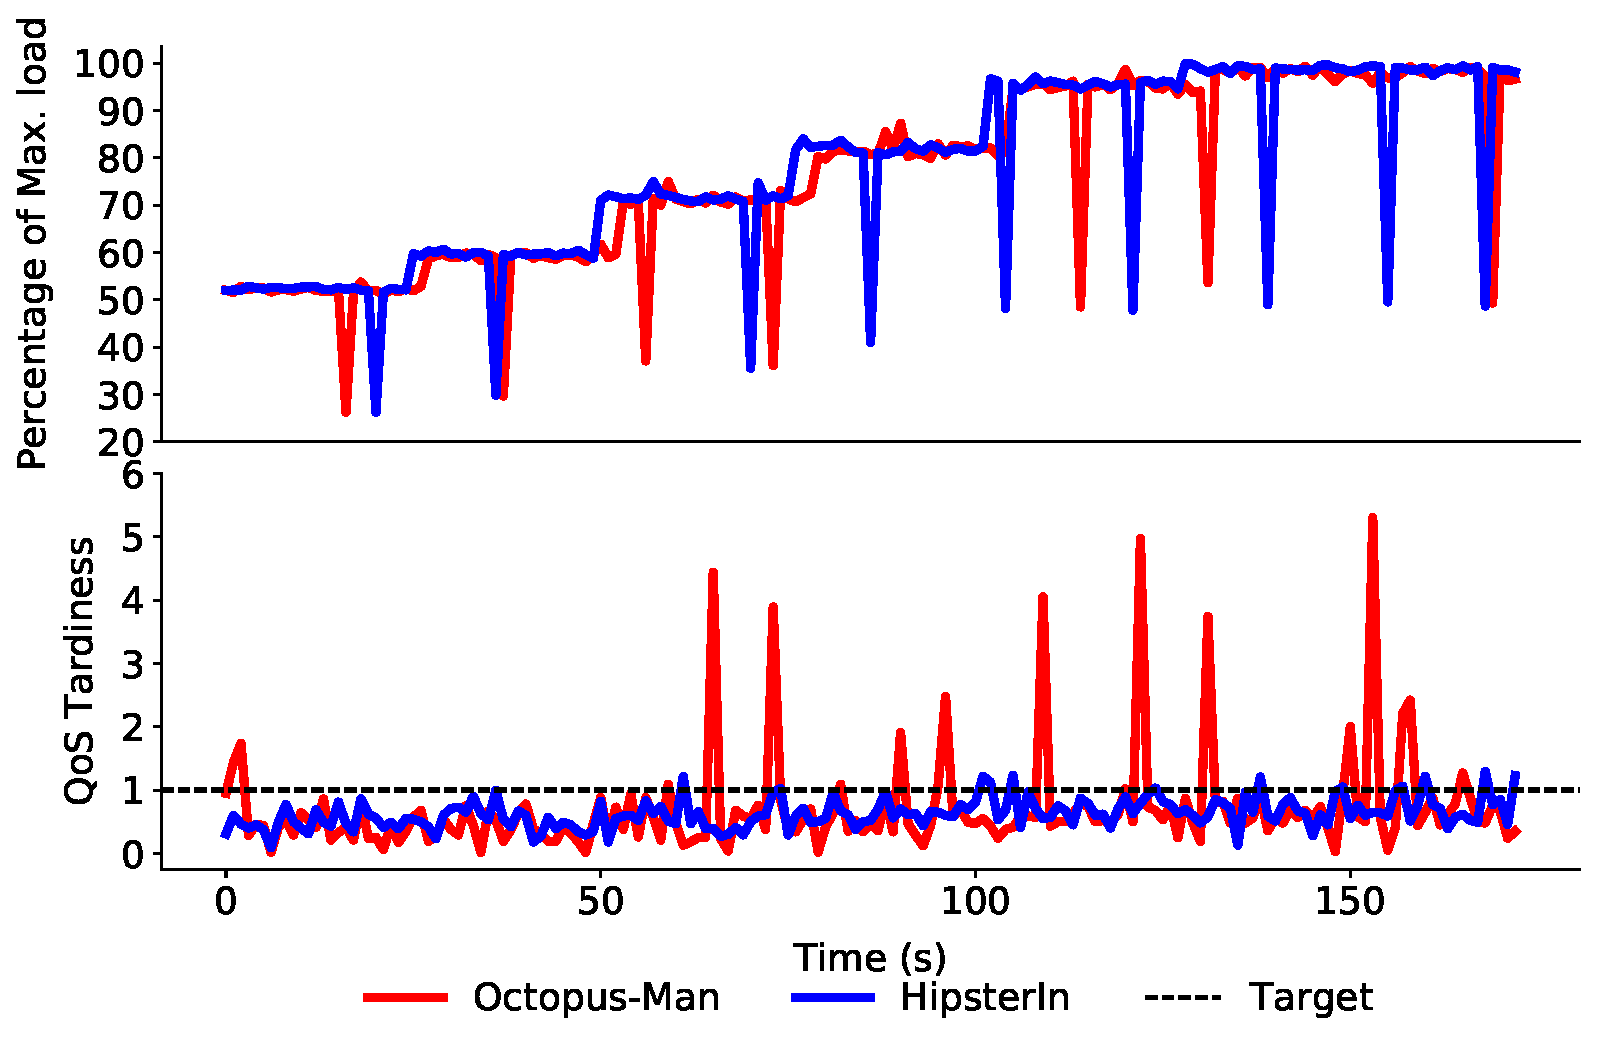
\includegraphics[width=0.7\linewidth]{Chapter4/Figs/detail_responsiveness.eps}
    \caption[Responsiveness to load change of HipsterIn and Octopus-Man]{\captitle{Responsiveness to load change of HipsterIn and Octopus-Man.} Percentage of Max. load, and Tail latency (QoS Tardiness) running Memcached with HipsterIn and Octopus-Man.}
	\label{fig: responsivenesstoloadchange}
\end{figure}



\paragraph*{Impact of learning time.} HipsterIn aims to deliver the best balance
between QoS guarantee and energy reduction compared to heuristic policies (Table~\ref{tab:
summarytable-hipster}). In practice, to best optimise for energy efficiency, and to improve QoS,
HipsterIn needs a short learning phase. Figure~\ref{fig: learningqos} shows the QoS
guarantee and energy distribution smoothed over \SI{100}{\second} intervals using the
Savitzky--Golay filter~\citep{Krishnan:2013:SOS:2710154.2710696} for Web-Search, for both
HipsterIn and Octopus-Man. Each data point in the graph refers to a 100-second interval.
The learning phase is set to \SI{200}{\second}. As can be seen, HipsterIn quickly learns
during the heuristic phase, which improves QoS guarantees. On the other hand, for
Octopus-Man, the QoS guarantees are consistently around the \SI{80}{\percent} mark, since
it does not use past decisions and their associated effects to improve the future
decisions. 

\begin{figure}[t]
    \centering
    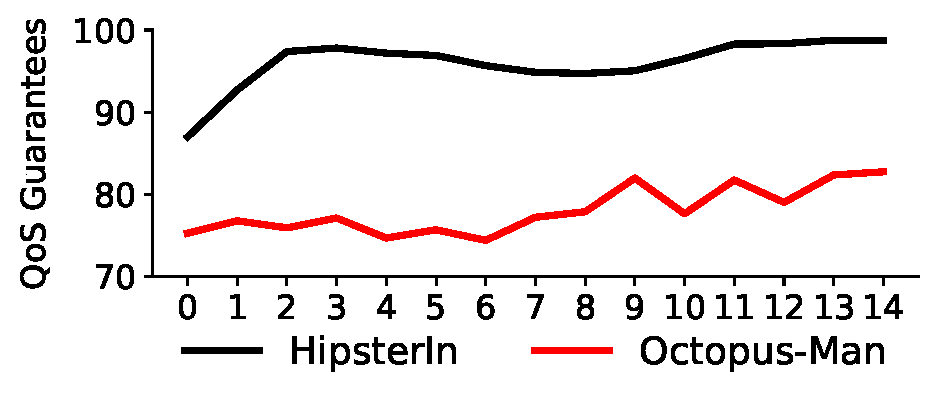
\includegraphics[width=0.8\linewidth]{Chapter4/Figs/learningqos.eps}
    \caption[QoS Guarantees of HipsterIn and Octopus-Man]{\captitle{QoS Guarantees of HipsterIn and Octopus-Man.} Each data point represents the QoS guarantees over \SI{100}{\second} intervals.}
    \label{fig: learningqos}
\end{figure}

\paragraph*{Impact of bucket sizes.} Figure~\ref{fig:loadbucket-qos-websearch} shows
the impact on QoS and energy savings when varying the load bucket sizes in Hipster. The
$x$-axis represents the bucket size, expressed as the percentage of maximum load. Each bar
in the figure ($y$-axis) represents the QoS violations and energy reductions normalised to
Static (all big cores). Using a large bucket size forces Hipster to use the same core
configuration across a wide range of loads, whereas using a small bucket size allows
fine-grained control. A small bucket size therefore improves the energy savings, but it
tends to cause rapid changes in core configuration for small changes in load, and doing so
incurs a larger number of QoS violations. On the other hand, larger bucket sizes provide
better QoS guarantee but lower energy savings, because they categorise large variations in
load into a single load bucket. Therefore, in tuning Hipster, we empirically determine the
bucket size to maximise energy savings subject to at least \SI{98}{\percent} QoS guarantee.

\begin{figure}[t]
\centering
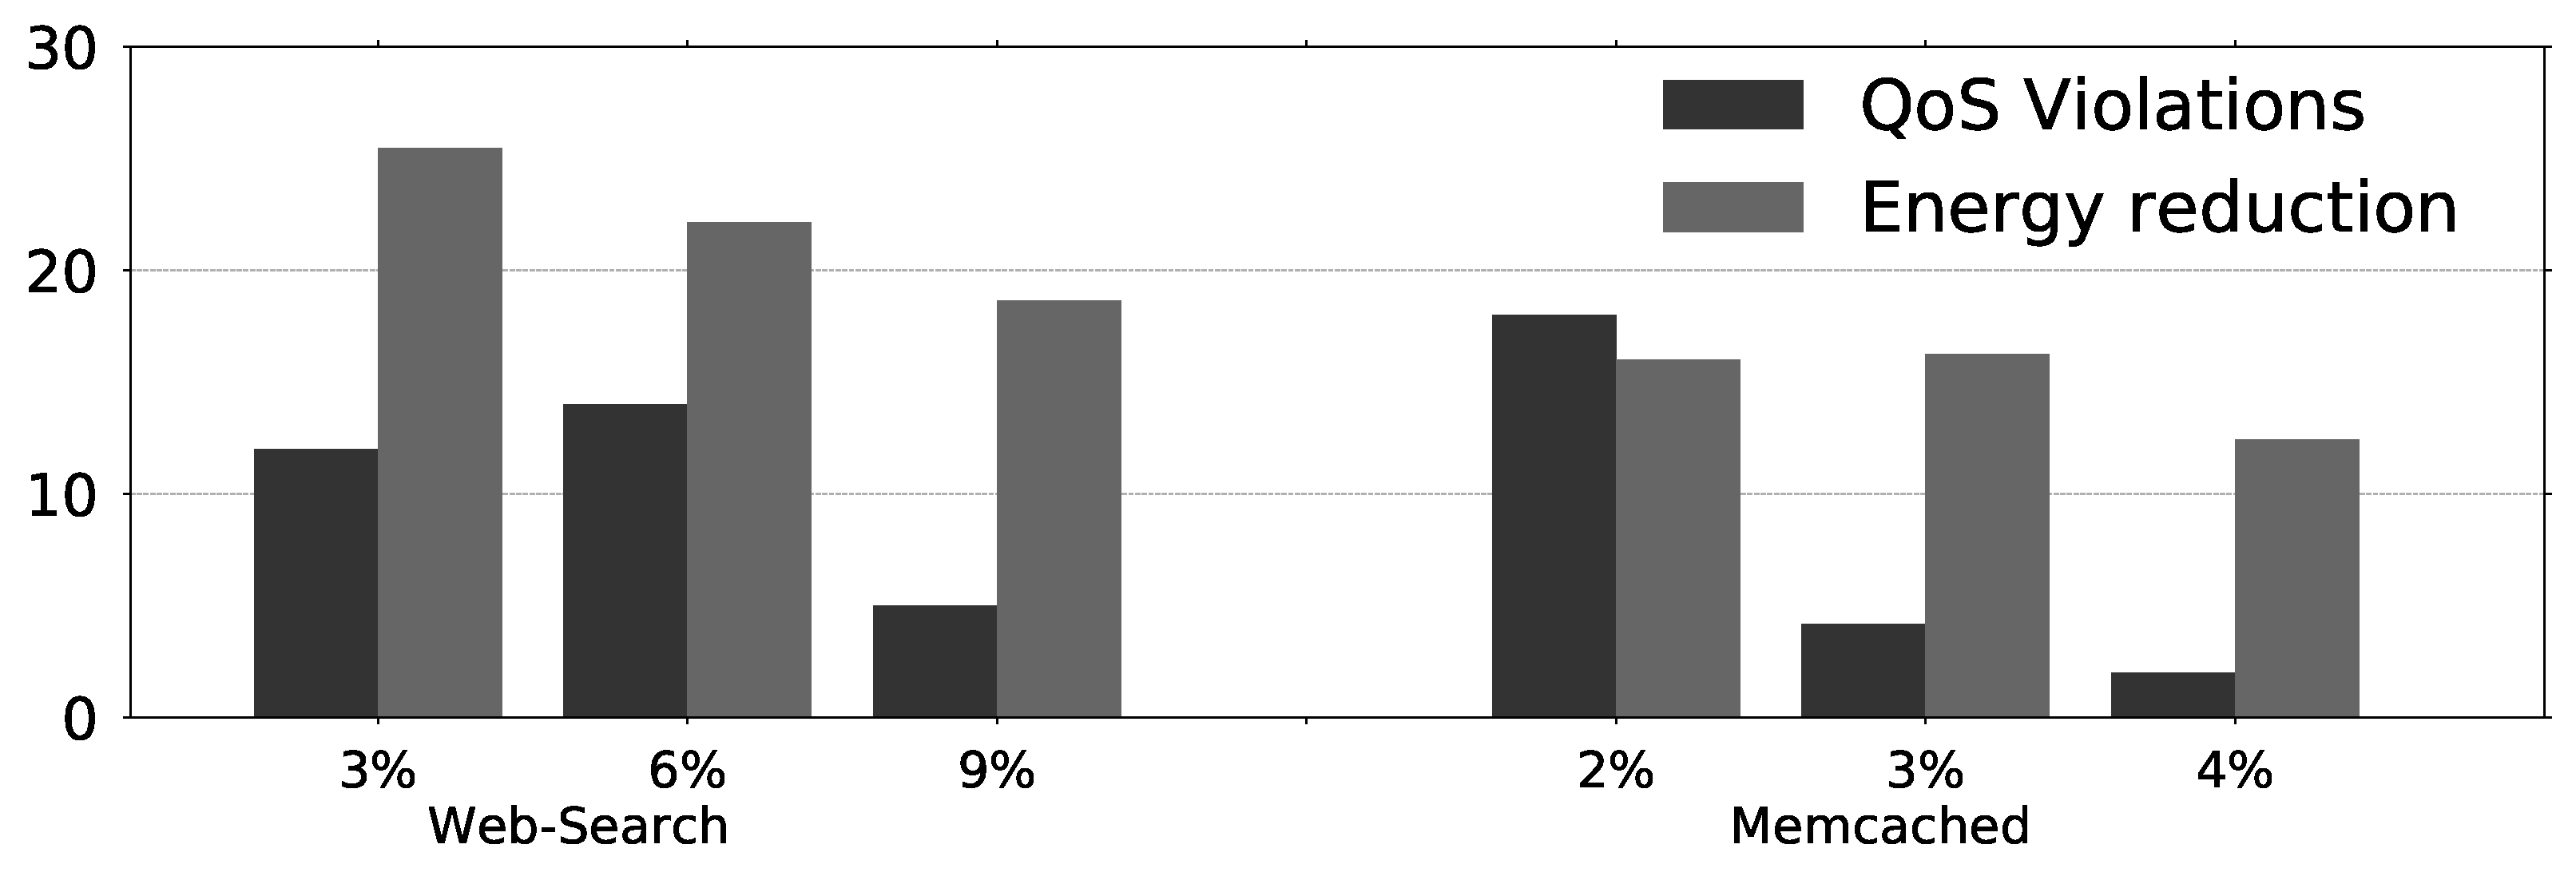
\includegraphics[width=0.95\linewidth]{Chapter4/Figs/bucketsize-qos-power.eps}
    \caption[Impact of bucket size on HipsterIn]{\captitle{Impact of bucket size.} QoS guarantees and energy savings normalised to static (all big cores) on Web-Search and Memcached.}
    %for HipsterIn QoS guarantees, and energy savings,normalised to static (all big cores) on Web-Search and Memcached.}
\label{fig:loadbucket-qos-websearch}
\end{figure}

\paragraph*{Optimising the lookup table size} Table~\ref{fig:sizehipster} summarises the
QoS guarantee, number of configurations per load bucket, and number of configurations for
Memcached and Web-Search with unoptimised and optimised lookup tables. We quantify the
reduction in lookup table size by assessing the number of configurations stored for each
load bucket at the end of the execution. As shown in Table~\ref{fig:sizehipster}, the
optimised lookup table saves \SI{90}{\percent} of the memory footprint while providing
similar QoS guarantee to unoptimised lookup table because, it only stores those
configurations that have been explored in the learning phase and in the exploitation
phase, the size of the table is further reduced by keeping only the top five
configurations with the highest reward. This is possible, as the configurations explored
at a given load level for a particular application are chosen from only a subset of the
configurations in the learning phase instead of random solutions as in Q-Learning.

\begin{table*}[t]
\centering
\ra{1.3}
\setlength{\tabcolsep}{5pt}
%{\def\arraystretch{2}\tabcolsep=10pt

    \caption{Results of the table size optimisation in Hipster} 
    \begin{tabular}{@{}llllr@{}}
        \toprule
                                                            &  Lookup Table           & Memcached	         & Web-Search  \\
        \midrule
        \multirow{2}{*}{QoS Guarantee (\%)}                 & Unoptimised    & 99.4                 & 96.5 \\
                                                            & Optimised      & 99.2                 & 96.0 \\
        \multirow{2}{*}{\# of config./load bucket}          & Unoptimised    & 13                   & 13  \\
                                                            & Optimised      & 5                    & 5 \\
        \multirow{2}{*}{Table size (elements)}              & Unoptimised    & 1344 (0\% savings)         & 392 (0\% savings) \\
                                                            & Optimised      & 120  (91.1\% savings)         & 35 (91.1\% savings)\\
                                                            
%        \multirow{2}{*}{Table Size in \SI{}{\kilo\byte}}    & Unoptimised    & 10.7                 & 10.7 \\
%                                                            & Optimised      & 0.9                  & 0.9 \\
        \bottomrule
    \end{tabular}    
    \label{fig:sizehipster} 
\end{table*}


\subsection{HipsterCo Results}
\label{subsec: coalloc}

\looseness -1 This section evaluates the effectiveness of HipsterCo, as a policy for
collocating a single latency-critical workload and a mix of batch workloads.  The
objective is to maximise the throughput of the batch workloads while satisfying QoS of the
interactive workloads.

Figure~\ref{fig:coallocaaaa} shows the QoS guarantee (top), throughput (middle) and energy
consumption (bottom) for Web-Search collocated with batch workloads, managed by
Octopus-Man and HipsterCo. All figures are normalised to a static mapping that allocates
the latency-critical workload to the two big cores and the batch workloads to the four
small cores. The number of running batch workloads is equal to the number of cores not
utilised by Web-Search. We report the system throughput by aggregating the IPS of all
batch programs. 

As shown in the top plot of Figure~\ref{fig:coallocaaaa}, HipsterCo consistently delivers
94\% QoS guarantees, whereas Octo\-pus-Man has much lower QoS guarantees of
\SI{76}{\percent}. This is because Hipster learns from the QoS behaviour and performance
history and is able to jump directly to a core mapping and DVFS state that satisfies QoS.
As a result, it incurs fewer core migrations compared with  Octopus-Man (see
Section~\ref{subsubsec: web-search results}), so it achieves superior QoS guarantees. 

\begin{figure}[ht]
    \centering
    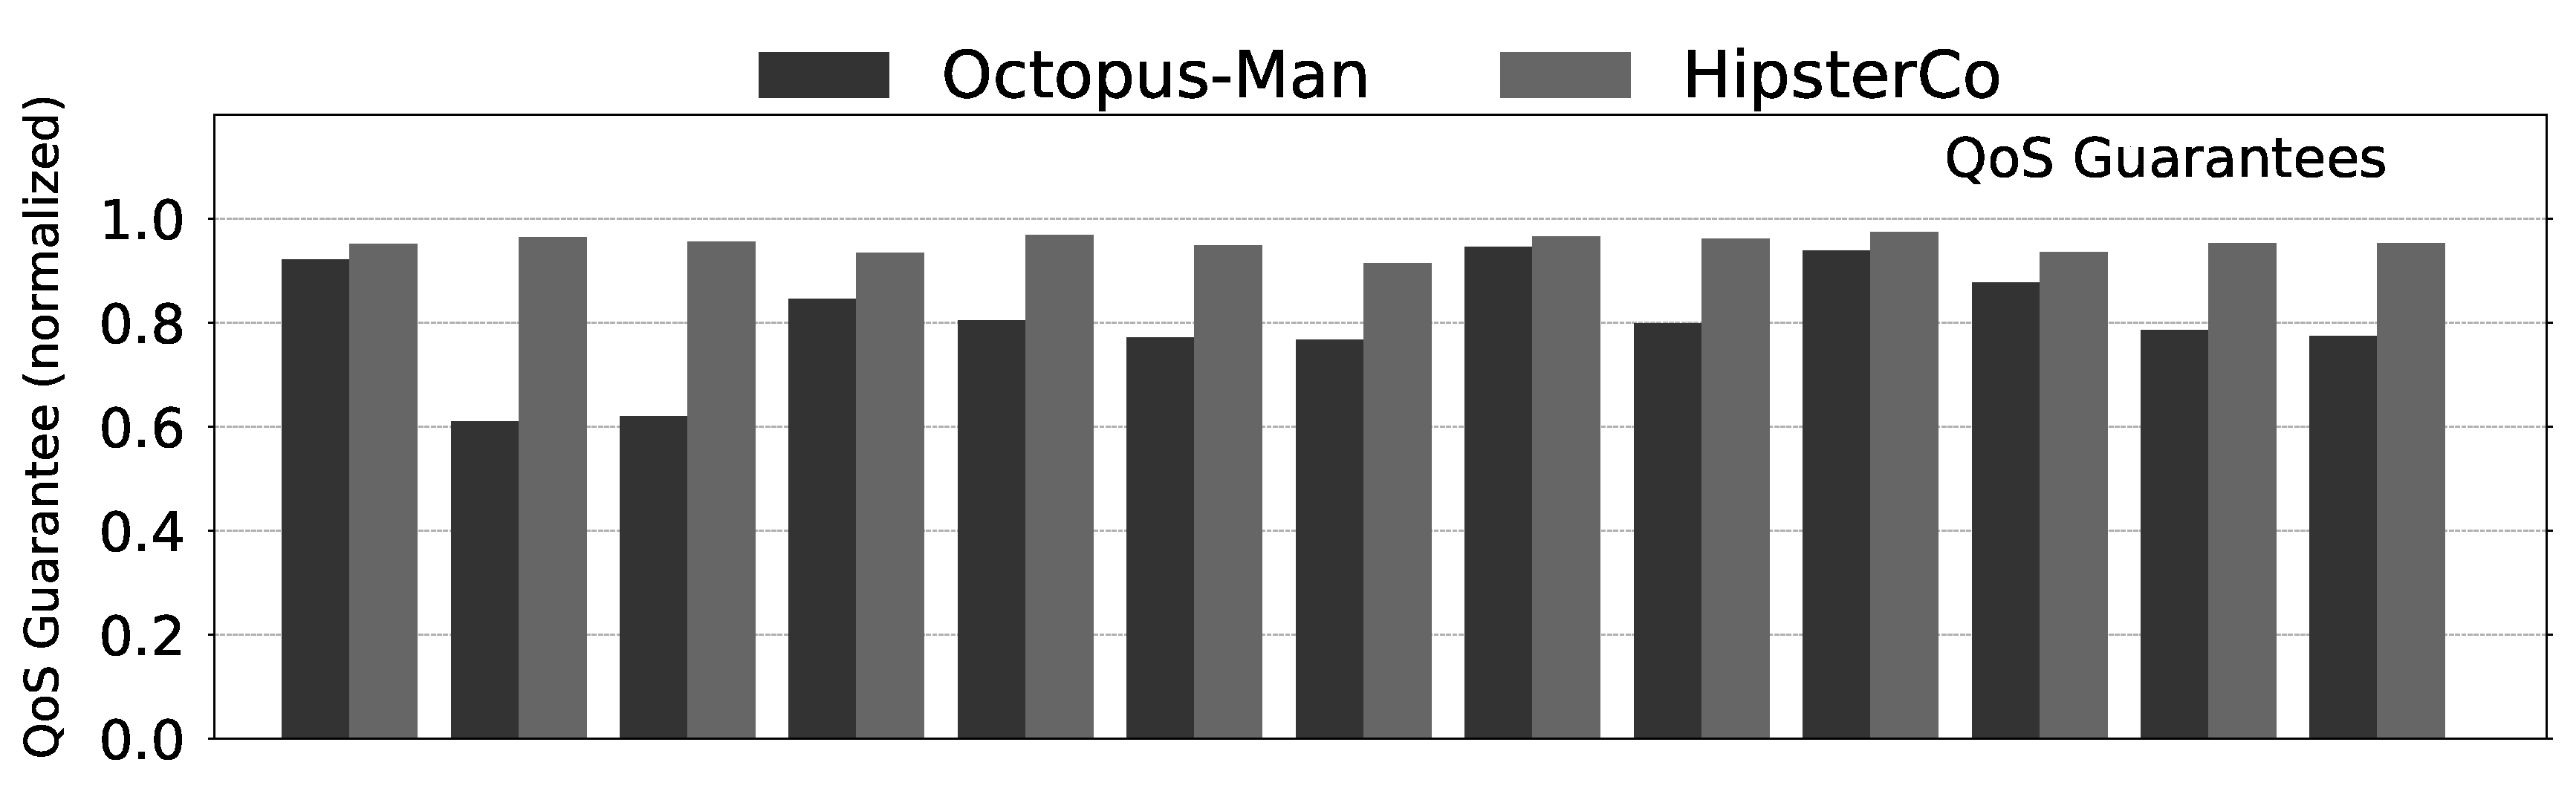
\includegraphics[width=0.9\linewidth]{Chapter4/Figs/guarantees_throughput_coalloc_without_yaxis.eps}
    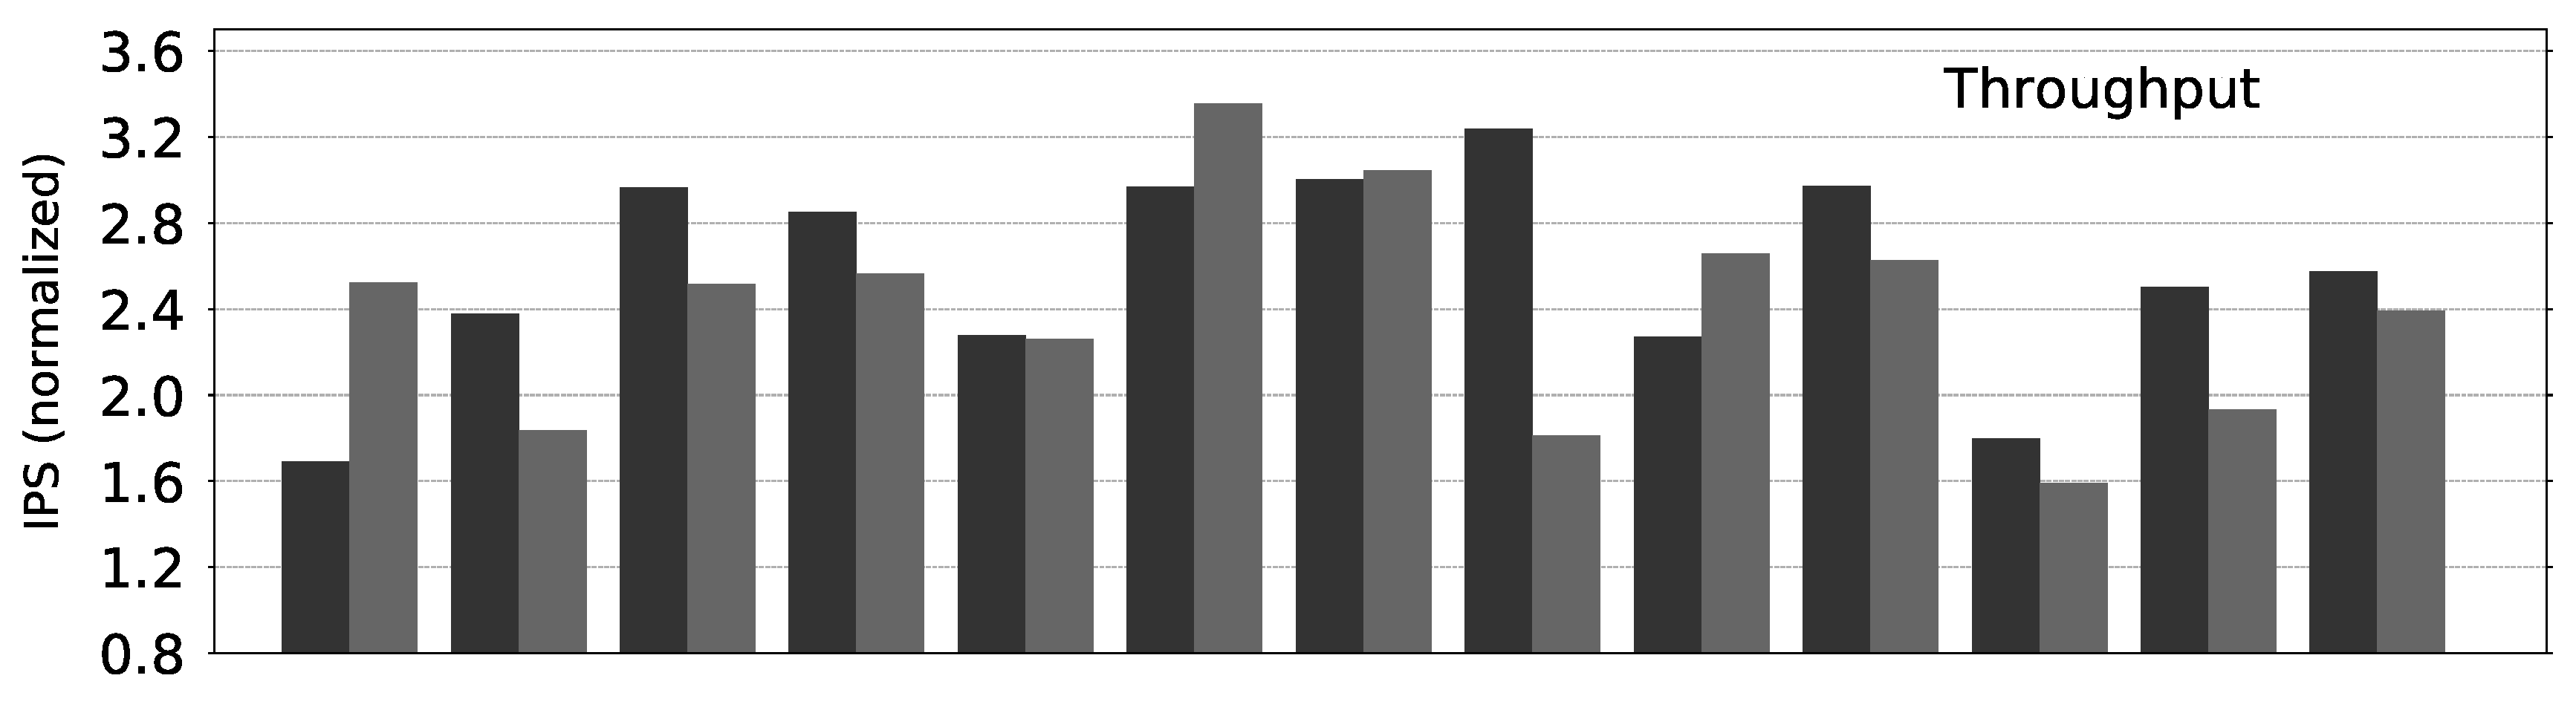
\includegraphics[width=0.9\linewidth]{Chapter4/Figs/throughput_coalloc_without_legend_axis.eps}
    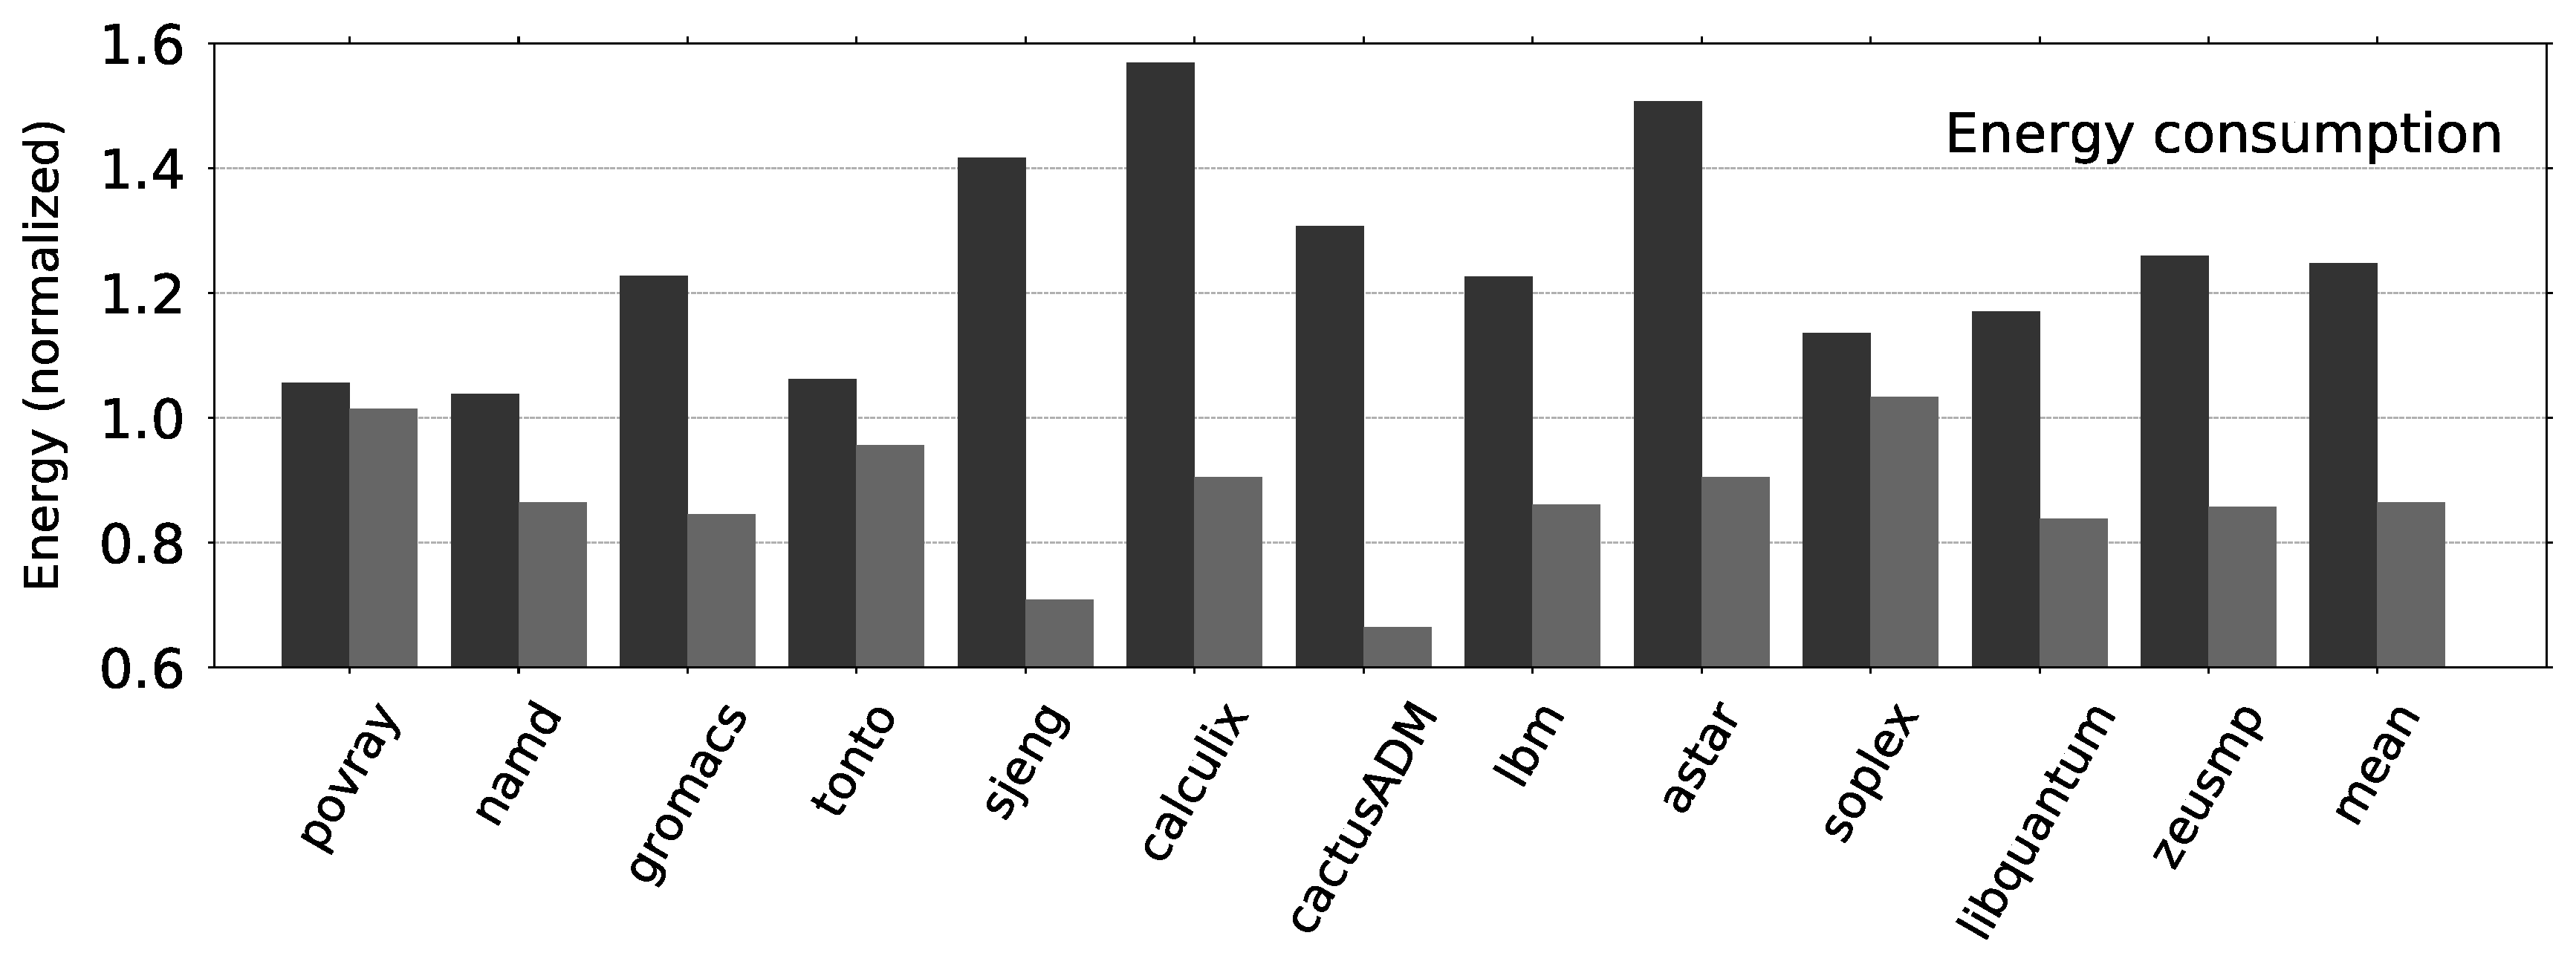
\includegraphics[width=0.9\linewidth]{Chapter4/Figs/energy_coalloc_withoutlegend.eps}

    \caption[Collocation of interactive and batch workloads with HipsterCo]{\captitle{Collocation of interactive and batch workloads with HipsterCo.} QoS guarantee (top), Throughput improvement (middle) and Energy consumption (bottom) when Web-Search is collocated with batch workloads. The results are normalised to static all big cores. }

\label{fig:coallocaaaa}
\end{figure} 

\looseness -1 As shown in the middle plot of Figure~\ref{fig:coallocaaaa}, for all
benchmarks, Hipster and Octopus-Man deliver much high\-er throughput compared to static
mapping, with an average of $2.3\times$ and $2.6\times$ improvement, respectively. Both
task managers improve performance compared with the static mapping because they migrate
the latency-critical workload to small cores during periods of low load, allowing the
batch workloads to run on big cores (which can be $2.6\times$ more powerful than small
cores).  For \emph{Calculix}, a compute-bound application, HipsterCo achieves the highest
throughput improvement over static of $3.35\times$, and for \emph{libquantum}, a
memory-bound program, the least improvement is still $1.6\times$.  

As shown in the bottom plot of Figure~\ref{fig:coallocaaaa}, HipsterCo reduces the energy
consumption to an average of \SI{80}{\percent} of static, whereas Octopus-Man increases
energy to an average of $1.2$ times that of static. This is because, as shown in
Figure~\ref{fig:octomancomp}, Hipster explores a wider range of core configurations,
including DVFS settings and mixing core types. In contrast, Octopus-Man only allows the
latency-critical workload to occupy a single cluster and each cluster is set to the
highest DVFS. 

HipsterCo sometimes chooses a different performance--energy trade-off than Octopus-Man.
An example is \emph{lbm}, a memory bound workload, for which HipsterCo delivers
\SI{40}{\percent} the throughput of Octopus-Man, but \SI{31}{\percent} lower energy.
There are two main reasons for this.  Firstly, when HipsterCo uses DVFS for the
latency-critical workloads, this DVFS setting also applies to batch workloads running in
the same cluster, reducing both batch throughput and system energy. Secondly, HipsterCo
sometimes uses a larger number of cores at lower DVFS, leaving fewer resources available
for the batch workloads. As a result, on average, HipsterCo marginally reduces performance
(by \SI{7}{\percent}) but it delivers energy savings of \SI{33}{\percent}, both compared
with Octopus-Man.

%\section{Hipster Implementation}
\label{sec: implementation}

Hipster is implemented in user space, and it uses minimal hardware support exposed by Linux. It consists of the QoS Monitor and Mapper Module, together with a lookup table, as shown in Figure~\ref{fig:hipsteroverview}. 

\looseness -2 \textbf{[QoS Monitor]:} Hipster uses a separate process to read the power measurements using native energy meters, at the sampling interval of the application. In addition to measuring energy, the QoS Monitor also gathers runtime statistics for the query/request latency of the latency-critical workload, using a logfile interface. In the case of HipsterCo, the  batch workload aggregate IPS per core are measured using the performance monitoring tool,
\textsf{perf}~\citep{2016Perf:Counters}, specifically using the \textit{perf\_event} \textsf{instructions}~\citep{ARMLimitedARMManual,ARMLimitedARMManualb}. Alternatives to \textsf{perf} include the profiling tools~\citep{Ren2010Google-WideCenters} supported by Docker, Kubernetes and LXC~\citep{Bernstein2014ContainersKubernetes}.  


On the ARM Juno platform, there is a known bug that causes \textsf{perf} to generate garbage values for all cores whenever any core enters an idle state. Since performance statistics are only needed for the HipsterCo variant, we overcome this by disabling CPUidle~\citep{ARMLimitedARMManual,ARMLimitedARMManualb}. This prevents Linux from entering the cores in an idle state when changes in the mapping cause idle periods longer than \SI{3500}{\micro\second}.

\textbf{[Mapper Module]:} The workloads are mapped to cores using the Linux \textsf{sched\_setaffinity} call and DVFS is controlled using \textsf{acpi-cpufreq}. In addition, Hipster suspends and resumes the batch workloads using the relevant OS signals ({\small \textsf{SIGSTOP}} and {\small \textsf{SIGCONT}} in Linux).

\textbf{[Lookup table]:} Each iteration of the RL algorithm accesses and modifies several entries in the lookup table. To ensure that these operations take negligible time, the computational complexity to access the table should be at most a few instructions. Therefore, in the prototype implementation of Hipster, the lookup table was implemented using a Python dictionary, which uses open addressing to resolve hash collisions, thereby having a computational complexity of $\mathcal{O}(1)$ irrespective of the operation~\citep{PattisComplexityHttps://www.ics.uci.edu/pattis/ICS-33/lectures/complexitypython.txt}.

%Using a tabular data structure to operate periodically would be very expensive ($\mathcal{O}(n\log{}n)$), but fortunately there are other data structures. For instance, $B-tree$ reduces the computational complexity for accesses, inserts or updates to $\mathcal{O}(\log{}n)$~\cite{GoetzModernTechniques}. In the prototype implementation of Hipster, we have it as a lookup table, but a $B-tree$ implementation is could reduce the complexity.

\section{Deployment Methodology for New Workloads} 
\label{sec: set hipster} 

\looseness -1 Hipster is a user-level daemon written in Python that is designed to
implement a hybrid reinforcement learning approach under Linux running on multicore
machines. It is released under General Public License (GPL) v3 and its source is available
for download.\footnote{https://bitbucket.org/rnishtala/hipster.git} To deploy Hipster at
runtime, we initiate a one-time system profiling to have minimal hardware understanding (similar
to Octopus-Man~\citep{Petrucci2015Octopus-Man:Computers}), and then the Hipster runtime is
responsible to manage a given workload on a physical machine. 

\subsection{System profiling} We profile the system by running the
stress microbenchmark (with no memory access) at different core mappings and DVFS settings
to gather the performance (such as IPS) and power statistics.\footnote{The stress
microbenchmark is executed on each of the available cores simultaneously and is given by ''stress\_cpu.c'' in the source code.} The performance and power
statistics can be obtained using performance monitoring tools (see section~\ref{subsec:
implementation}) and power meters (see section~\ref{sec: power meters}), respectively.
Then, sort the configurations in the increasing order of the system's mean power
efficiency (performance per watt of power consumed) and only the order is of interest to
us. The system's TDP is obtained by running the microbenchmark on all cores at the highest
DVFS setting. 

For each (new) latency-critical workload, we quantify the maximum load (measured in terms
of queries/requests per second or similar) the system can manage on the most
power efficient configuration while satisfying the QoS target (measured in
\SI{}{\milli\second} or \SI{}{\second}).

\vspace{1mm}

\subsection{Hipster runtime} Hipster is invoked periodically, with the period determined by
the sampling interval of the latency-critical workload. Hipster takes as input the
\textit{system power consumption}, \textit{QoS target}, \textit{load}, \textit{maximum
load} and \textit{latency} (measured in \SI{}{\milli\second} or \SI{}{\second}) of the
latency-critical workload and finally, the \textit{performance} (measured in IPS) of the
throughput-oriented workload (if any). The performance metrics such as QoS target, load and
latency can be obtained either from the application directly (as in our case) or an external profiling tool
such as Google Wide Profiler (GWP)~\citep{Ren2010Google-WideCenters}.

\looseness -1 To make the best use of Hipster, we suggest tuning the upper
 threshold ($QoS_{\mathit{D}}$) and lower  threshold ($QoS_{\mathit{S}}$), learning factor
($\xi$), discounting factor ($\gamma$) empirically. Nevertheless, in the current
implementation, we predefine the upper threshold and lower threshold to  80\% and 20\% of the QoS
target, respectively; and the learning factor and discounting factor are set to 0.6 and
0.9, respectively. 

Our implementation assumes that there exists an ACPI governor~\citep{ondemand} that allows external changes to DVFS state. The governor selected
on our ARM processor is \textsf{userspace}. The deployment stage of Hipster needs
permission to access \textsf{Ring 0} or \textsf{root} as the ACPI module writes
changes in DVFS state to the \textsf{sysfs}. We provide an example of Hipster's deployment method. 

\vspace{1mm}

Hipster schedules the workloads using Hipster's heuristic algorithm and reinforcement
learning mechanism. For a multicore server, we use Hipster to dynamically select the core
mapping and DVFS state to ``just meet'' the QoS based on the load for an interactive
workload and any remaining resources are allocated to throughput-oriented workloads (if
any).
 

\section{Conclusion}
\label{sec: conclusion-hipster}

\looseness -1 We propose Hipster, a hybrid scheme that combines heuristics and
reinforcement learning to manage heterogeneous cores with DVFS control for improved energy
efficiency. We show that Hipster performs well across workloads and interactively adapts
the system by learning from the QoS/power/performance history to best map workloads to the
heterogeneous cores and adjust their DVFS settings.  When only latency-critical workloads
are running in the system, Hipster reduces energy consumption by \SI{13}{\percent} in
comparison to prior work. In addition, to improve resource efficiency in shared data
centres by running both latency-critical and batch workloads on the same system, Hipster
improves batch workload throughput by $2.3\times$ compared to a static and conservative
policy, while meeting the QoS targets for the latency-critical workloads.

